%%%%%%%%%%%%%%%%%%%%%%%%%%%%%%%%%%%%%%%%%%%%%%%%%%%%%%%%%%%%%%%%%%%%%%%
%% Optionen zum Layout des Buchs                                     %%
%%%%%%%%%%%%%%%%%%%%%%%%%%%%%%%%%%%%%%%%%%%%%%%%%%%%%%%%%%%%%%%%%%%%%%%
\documentclass[
a4paper,							% alle weiteren Papierformat einstellbar
%landscape,						% Querformat
11pt,								% Schriftgr��e (12pt, 11pt (Standard))
%BCOR1cm,							% Bindekorrektur, bspw. 1 cm
%DIVcalc,							% f�hrt die Satzspiegelberechnung neu aus
%											  s. scrguide 2.4
%oneside,							% einseitiges Layout
%twocolumn,						% zweispaltiger Satz
%openany,							% Kapitel k�nnen auch auf linken Seiten beginnen
%halfparskip*,				% Absatzformatierung s. scrguide 3.1
%headsepline,					% Trennline zum Seitenkopf	
%footsepline,					% Trennline zum Seitenfu�
%notitlepage,					% in-page-Titel, keine eigene Titelseite
%chapterprefix,				% vor Kapitel�berschrift wird "Kapitel Nummer" gesetzt
%appendixprefix,				% Anhang wird "Anhang" vor die �berschrift gesetzt 
%normalheadings,			% �berschriften etwas kleiner (smallheadings)
%idxtotoc,						% Index im Inhaltsverzeichnis
%liststotoc,					% Abb.- und Tab.verzeichnis im Inhalt
%bibtotoc,						% Literaturverzeichnis im Inhalt
%bibtotocnumbered,			% Nummerierstes Literaturverzeichnis im Inhalt 
%leqno,								% Nummerierung von Gleichungen links
%fleqn,								% Ausgabe von Gleichungen linksb�ndig
%draft,								% �berlangen Zeilen in Ausgabe gekennzeichnet
titlepage,
pdftex
]
{scrreprt}
%{scrartcl}


\newcommand{\todo}[1]{    
	\addcontentsline{tdo}{todo}{\protect{#1}}    
	\marginpar{\textbf{\textcolor{red}{#1}}}
	}
\makeatletter \newcommand \listoftodos{\section*{Todo Liste} \@starttoc{tdo}}  \newcommand\l@todo[2]    {\par\noindent \textit{#2}, \parbox{10cm}{#1}\par} 


\setcounter{secnumdepth}{4}
\setcounter{tocdepth}{4}

\usepackage[ngerman, final]{hyperref}
\usepackage[ngerman]{babel}
\usepackage[T1]{fontenc}       
\usepackage[latin1]{inputenc}
%\usepackage{graphicx}
\usepackage{multicol}
\usepackage{amsmath}
%\usepackage[mediumspace,mediumqspace,Grey,squaren]{SIunits}
%\usepackage{multirow}
\usepackage{color,listings}
\usepackage{ltxtable}
\usepackage{longtable}
\usepackage{tabularx}
\usepackage{multirow}
\usepackage{lscape}
\usepackage{pdfpages}
\usepackage{array}


\lstset{language=Java, % Grundsprache ist C und Dialekt ist Sharp (C#)
captionpos=b, % Beschriftung ist unterhalb
frame=lines, % Oberhalb und unterhalb des Listings ist eine Linie
%basicstyle=\ttfamily, % Schriftart
basicstyle=\small, % Schriftart
keywordstyle=\color{blue}, % Farbe f�r die Keywords wie public, void, object u.s.w.
commentstyle=\color{green}, % Farbe der Kommentare
stringstyle=\color{red}, % Farbe der Zeichenketten
numbers=none, % Zeilennummern links vom Code
numberstyle=\tiny, % kleine Zeilennummern
numbersep=5pt,
breaklines=true, % Wordwrap a.k.a. Zeilenumbruch aktiviert
showstringspaces=false,
% emph legt Farben f�r bestimmte W�rter manuell fest
emph={double,bool,int,unsigned,char,true,false,void},
emphstyle=\color{blue},
emph={Assert,Test},
emphstyle=\color{red},
emph={[2]\using,\#define,\#ifdef,\#endif}, emphstyle={[2]\color{blue}}
}

\hypersetup
{
pdftitle = {GPicS},
pdfsubject = {GPicS},
pdfauthor = {Rico Scholz,Stefan Radusch,Martin Schicht,Markus Ullrich},
pdfkeywords = {XML,GPicS,Fotoarchiv},
colorlinks = {false},
pdfborder = 0 0 0
}
\urlstyle{same}
\title{GPicS}
\subtitle{Entwicklung eines XML basierten Fotoarchiv}
\author{Rico Scholz\\IIAm10 \\ Fachbereich Informatik \\
Hochschule Zittau / G�rlitz
\and Stefan Radusch\\IIAm10 \\ Fachbereich Informatik \\
Hochschule Zittau / G�rlitz
\and Martin Schicht\\IIAm10 \\ Fachbereich Informatik \\
Hochschule Zittau / G�rlitz
\and Markus Ullrich\\IIAm10 \\ Fachbereich Informatik \\
Hochschule Zittau / G�rlitz}
\date{Lehrveranstaltungsleiter:\\
Prof. Dr. rer. nat. Cristian Wagenknecht\\
\bigskip\today}
	
\begin{document}
	\newcommand{\markiert}{\bf\emph}
	\renewcommand{\figurename}{Abbildung}
	\renewcommand{\refname}{B�cher}
%	\addto\captionsngerman{\renewcommand{\abstractname}{\Large{Zusammenfassung}}}
	\newenvironment{nosepitemize}{\begin{itemize}\itemsep 0pt}{\end{itemize}}
	\newcolumntype{C}[1]{>{\centering\arraybackslash}m{#1}}
	\maketitle

	\tableofcontents
	\listoffigures
	\listoftables
	\lstlistoflistings
	\listoftodos
	\newpage
	\begin{abstract}
	\normalsize{Diese Arbeit befasst sich mit der Erstellung eines XML basierten Fotoarchivs...}
\end{abstract}
	\chapter{Einleitung}
\label{JumpEinleitung}
In dieser Belegarbeit wird die Entwicklung einer Webanwendung unter Verwendung von XML-Technologien beschrieben. Als Fallbeispiel wurde daf�r die Erstellung eines Online-Fotoarchivs gew�hlt. Die konkrete Aufgabenstellung ist auf der n�chsten Seite beschrieben. Nach der Analyse dieser, wurde ein bestehendes Content Management System\footnote{kurz: CMS} namens Drupal auf die Anforderungen hin untersucht. Als Ergebnis stand fest, dass es nicht gen�gend den Anforderungen entspricht und somit eine Neuentwicklung von N�ten ist. Im Kapitel Technologien auf Seite \pageref{JumpTechnologien} ff, wurden die verwendeten Frameworks vorgestellt. Nach der Beschreibung der Entwicklungsumgebung, die aus dem Servlet-Container Tomcat, dem Continuous Integration Server Hudson,  der IDE IntelliJ und GoogleCode besteht, folgt im Kapitel \ref{JumpSystementwurf} der Systementwurf. Auf diesen aufbauend schlie�t sich die Implementation an. Diese erstreckt sich von der Datenbank, �ber die einzelnen Seitencontroller und der Beschreibung wie die Frameworks verwendet wurden, bis hin zur Erl�uterung wie die Benutzeroberfl�che erstellt wurde. Anschlie�end folgt das Kapitel Tests, welches die Vorgehensweise zum Testen der einzelnen Komponenten beschreibt. Daran f�gt sich die Beschreibung, wie die Aufgabe unter den 4 Projektmitgliedern aufgeteilt wurde und mit welcher Absicht, an. Abschlie�end wird eine Zusammenfassung �ber das Projekt gegeben.
	\chapter{Problem}
\label{JumpProblem}
\section{Aufgabenstellung}
\label{JumpAufgabenstellung}
Das Ziel des Projektes ist es, ein Online-Foto-Archiv zu entwickeln, in dem Benutzer Bilder ins Internet stellen k�nnen. Dabei soll es eine M�glichkeit geben, um zu entscheiden, welche �ffentlich oder nach einer Authentifizierung zug�nglich sind. Mehrere Fotos sollen zu einem Album zusammengefasst und gesammelt angezeigt werden k�nnen. Weiterhin sollen Metainformationen aus den Bildern extrahiert und bearbeitet werden k�nnen. Diese sollen in geeigneter Form, z.B. einer Karte der Region, wo sie aufgenommen wurden, dargestellt werden.\newline\newline
Daf�r sollten eine Reihe von Technologien genutzt und evaluiert werden. Dazu geh�ren die Frameworks Primefaces und JSF, die Dateiformate JPEG und KML, die Entwicklungsumgebung IntelliJ, sowie verschiedene Webservices zur Nutzung von GoogleMaps. 
\section{Anforderungsanalyse}
\label{JumpAnforderungsanalyse}
	\chapter{Evaluation eines bestehenden Systems - Drupal}
\label{JumpDrupal}

Viele Menschen wollten schon immer ihre eigene Website, ihren Blog, ihr Forum oder ähnliches haben, doch sind immer an den HTML- und Programmierkenntnissen gescheitert. Das ist seit dem Beginn von Content-Management-Systemen (CMS) vorbei. Solche Systeme ermöglichen es in den meisten Fällen ohne Programmier- und HTML-Kenntnisse eine Website im Handumdrehen zu erstellen. Bei einigen Webspaces oder Online-Hostern sind solche Systeme schon bereits vorinstalliert und können schnell und einfach genutzt werden oder sie sind dafür geeignet und man muss sein CMS nur dort hochladen. Zu den bekanntesten Content Management Systemen zur Zeit zählen Typo3, Joomla und mittlerweile auch Drupal. Da Drupal immer stärker im kommen ist und einen immer größer werdenden Zuwachs findet, wird Drupal im nächsten Abschnitt mal etwas genauer beleuchtet werden. \\
\\
Drupal ist ein CMS und Framework, welches ursprünglich vom belgischen Informatiker Dries Buytaert entwickelt wurde. Es handelt sich dabei um eine freie Software, die unter der General Public License (GNU) steht. \\
\\
Wer Drupal nutzen möchte benötigt dafür lediglich einen Webserver, auf dem sich PHP und eine SQL-fähige Datenbank befindet. Das sind alles Dinge, die die meisten Webspaces kostenlos oder für einen kleinen Preis zur Verfügung stellen. PHP ist eine Skriptsprache, die hauptsächlich zur Erstellung dynamischer Webseiten oder Webanwendungen verwendet wird. Sie wird deshalb benötigt, da Drupal in PHP programmiert wurde.\\
\\
Der Aufbau von Drupal ist sehr einfach und lässt sich wie folgt beschreiben. Drupal besteht aus zwei Teilen, einem Core(Kern) und Modulen. Der Core beinhaltet die Grundfunktionalität, welche mit weiteren Modulen erweitert werden kann. Zur Grundfunktionalität zählen Komponenten wie Template-Erstellung, Blogsystem, Benutzerverwaltung und Taxonomie. Diese Core-Funktionen reichen aus um eine simple Website zu erstellen. Man kann mit Hilfe der Template-Erstellung festlegen in welchen Bereichen der Website welcher Content angezeigt werden soll und auch die farbliche Gestaltung der gesamten Seite definieren. Die Benutzerverwaltung von Drupal ist sehr ausführlich und detailliert. Sie zieht sich über mehrere Seiten und man kann dort Benutzergruppen definieren und ihnen Rechte zuweisen. Die Rechte können von Artikelarten die ein Benutzer schreiben darf, über die Bilderanzahl pro Artikel bis hin zu Kommentarfunktion und vielen mehr gehen. Mit hilfe von Taxonomie lassen sich Menüs erstellen und verschiedene Artikel bzw. Beiträge der Website einer Kategorie zuweisen. Das kann über vorkommende Begriffe in Beiträgen oder über eine Auswahl der Kategorie beim Schreiben des Artikels passieren. \\
\\
Der andere Teil neben dem Core sind die Module. Die sind dafür da um je nach Anforderung Funktionen nachzurüsten. Diese Module werden meist von anderen Nutzer geschrieben und stehen dann allen zur Verfügung und können per Download integriert werden.
Was dabei zu beachten ist, ist die Menge der Module. Es gibt eine sehr große Anzahl und man kann nicht immer gleich am Modulnamen erkennen, was dieses Modul kann bzw. welche Funktion es liefern soll. Zudem wurde in mehreren Test festgestellt, das viele Module noch nicht richtig Funktionieren und sich oft noch im Beta-Status befinden.\\
\\
So muss man als Fazit sagen, dass Drupal eine echte Alternative in Sachen CMS ist zur schnellen und einfachen Erstellung einer Website oder eines WebBlogs, aber im Hinblick auf die Erstellung eines Foto-Archivs noch als eher ungeeignet darstellt. Da viele Funktionen die man in einem Foto-Archiv erwartet, wie eine Diashow oder eine Albumübersicht, Übersicht der Bilder nur schwer bis gar nicht realisieren lassen. Das liegt daran, dass dafür weitere Module benötigt werden, die zahlreich vorhanden sind, aber leider nicht zusammen arbeiten. So kann es sein das man nach langem Suchen ein passendes Modul finden aus der Vielzahl der Module, diese aber dann nicht mit den weiteren benötigten Modulen funktionieren. Das kommt daher, das jeder der sich mit Programmierung auskennt, sein eigenes Modul schreiben und veröffentlichen kann. Da aber jeder sein Modul so schreibt, dass es für seine Zwecke funktioniert, kommt es immer wieder zu Konflikten untereinander.

	\chapter{Verwendete Technologien}
\label{JumpTechnologien}
\section{Primefaces}
\label{JumpPrimefacesTechnologien}
\subsection{Allgemeines}
In heutigen Webanwendungen werden h�ufig viele Technologien verwendet um eine ansprechende Benutzeroberfl�che zu realisieren. Da gewisse Anforderungen immer wieder auftreten, wie zum Beispiel ein Dateiupload, ist es w�nschenswert ein Framework zu verwenden. Wie in Abschnitt \ref{JumpJSF} erl�utert wird, ist das Basis-Framework f�r dieses Projekt JSF. Mit diesem k�nnen zwar grunds�tzlich alle Anforderungen erf�llt werden (u.a. Dateiupload), doch es ist immer eine Erleichterung, wenn es daf�r schon vorgefertigte Komponenten gibt. In diesem Projekt wird Primefaces verwendet. Damit k�nnen alle Anforderungen schnell umgesetzt werden.\\
\\
Au�erdem soll nat�rlich die Benutzeroberfl�che immer ansprechend gestaltet sein. Bei Primefaces sind die Komponenten schon mit einem h�bschen Design vorhanden. Dieses vorgefertigte Design muss nicht unbedingt einen Nachteil bieten, und in diesem Projekt ist es auch kein Nachteil, da dadurch ein aufwendiger Designentwurf f�r diese Komponenten entfallen konnte. Es ist sogar m�glich dieses Design ein wenig zu beeinflussen.\\
\\
Wie jeder wei� gibt es nat�rlich eine ganze Reihe solcher Frameworks, die einen das Leben erleichtern. An dieser Stelle w�ren unter anderem RichFaces und IceFaces zu nennen. Aber unsere Wahl ist trotzdem auf Primefaces gefallen, weil es zum Einem eine Anforderung war Primefaces zu nutzen und zum Anderem bietet Primefaces n�tzliche Funktionen f�r dieses Projekt. So bietet Primefaces bereits eine Komponente f�r die Einbindung einer GoogleMaps-Karte. Mit dieser Komponente ist es au�erdem m�glich, Bilder in eine GoogleMaps-Karte anzuzeigen. Mit Primefaces ist es m�glich die Kernanforderung, ein Fotoarchiv zuerstellen, das Bilder in einer GoogleMaps-Karte anzeigen kann, umzusetzen. Dies erspart eine aufwendige Neuentwicklung.\\
\\
Primefaces wird in diesem Projekt in der Version 2.2.1 verwendet. Dies ist die aktuelle stabile Version. Im Moment befindet sich die Version 3 in Entwicklung und es gibt auch schon Vorabversionen davon. Es wurde trotzdem die Version 2.2.1 verwendet, da einige Projektmitglieder bereits schlechte Erfahrungen mit Vorabversionen in anderen Projekten gemacht haben.
\section{Evaluierung Primefaces}
\label{JumpPrimefacesEval}
Unsere Erfahrung mit dem Framework Primefaces l�sst sich sehr gut in einem Satz zusammenfassen, dieser lautet: "`Einfach zu implementieren, schlecht zu personalisieren."'. Zu Beginn stellten sich sehr schnell Erfolge ein, besonders das Showcase auf der Projektseite\footnote{\url{http://www.primefaces.org/showcase/ui/home.jsf}} bietet Einsteigern genug Informationen und Anschauungsmaterial f�r eigene Umsetzungen. Durch die ebenfalls sehr gute und ausf�hrliche Beschreibung im Handbuch, die das Showcase erg�nzte, konnten weitere Komponenten in das eigene Projekt integriert werden. Jedoch gelangt man irgendwann zu dem Punkt, an dem Mann den Weg des Showcase verlassen muss und auf Grund der eigenen Anforderungen Dinge anders implementieren muss. Besonders bei der Verwendung von dynamischen Bildern, also Bildern die nicht im Web-Ordner abgelegt sind, sondern via Streamed Content geladen werden, verh�lt sich Primefaces nicht wie erwartet. Auf Grund der Tatsache, dass man wenig Feedback per Fehlermeldungen bekommt, sieht man nur, dass etwas nicht funktioniert hat, aber nicht wo der Fehler ist. Bez�glich dieser Bilder gibt es noch einen weiteren Kritikpunkt. Immer wenn solche Objekte geladen werden, f�hrt Primefaces mindestens drei Requests aus, beobachtet wurden bis zu sechs. Bei einem Controller der einen Request Scope besitzt bedeutet dies, dass genauso viele neue Controller initialisiert werden und trotzdem die R�ckgabe des Bildes nicht funktioniert hat. Deshalb mussten fast alle Controller die mit Primefaces-Komponenten in Verbindung stehen mit Session Scope ausgestattet werden. Dies f�hrt zu den bekannten Seiteneffekten, die beachtet werden m�ssen.\newline\newline
Als positve Punkte sind zu erw�hnen, dass Primefaces eine Vielzahl von Komponenten bereitstellt und diese eine breite Palette von Aufgabenstellungen abdecken. Des Weiteren ist das Design der sehr modern und kann zus�tzlich noch angepasst werden.\newline\newline
Insgesamt l�sst sich sagen, dass Primefaces sehr viel bietet und man schnell zu Ergebnissen kommt. Bei multimedialen Inhalten sind, bei der getesteten Version 2.2.1, gr��ere Schw�chen zu erkennen und daher bei diesen Aufgaben nicht zu empfehlen. Sollte man diese aber nicht ben�tigen ist Primefaces ein leichtgewichtiges Framework, welches schnell zum Ziel f�hrt. Da das Projekt weiterentwickelt wird und mit einem Milestone der Version 3 bereits eine Weiterentwicklung zur Verf�gung steht, sollte beobachtet werden, wie diese in Bezug auf Medien erweitert wird.
\section{JSF}
\label{JumpJSF}
Schon immer wird in der Programmierung versucht bestehendes wiederzuverwenden. Dieser Ansatz findet sich auch in der Programmierung von Web-Applikationen. F�r die Programmierung von Web-Applikationen ist so ein Framework JSF. Dieses Framework basiert auf Servlets und JSPs und bietet eine gute M�glichkeit komfortabel Webseiten zu entwickeln.\\
\\
Nat�rlich gibt es noch weitere Frameworks, so dass die Frage im Raum steht warum in diesem Projekt JSF als Basis-Framework verwendet wird. Zum einem w�re hier zu nennen, dass JSF schon eine Weile auf dem Markt ist, was f�r die Programmierung einen gro�en Vorteil darstellt. Es geht nichts �ber eine gute Dokumentation eines Frameworks. Au�erdem gibt es im Internet fast immer eine L�sung f�r ein Problem, da fast immer jemand anderes vorher das Problem auch hatte. Durch diesen Vorteil konnte die Entwicklung beschleunigt werden.\\
\\
Ein weiterer Grund f�r die Verwendung von JSF ist die Anforderung des Auftraggebers. Dieser hat vorgeschlagen das Projekt mit JSF zu verwirklichen. Da dies aus oben genannten Gr�nden ein guter Vorschlag war, wurde JSF verwendet.\\
\\
In diesem Projekt wird die Version 2.0.1 von Mojarra verwendet. Sie bietet eine gute Unterst�tzung f�r Facelets und ist im Moment die aktuelle Version von JSF. Die Version von Mojarra bietet die gleichen Funktionalit�ten wie die Referenzimplementierung von Apache MyFaces. Der Grund f�r die Verwendung von Mojarra ist darin begr�ndet, dass die IDE bei der Entwicklung Mojarra als einzige M�glichkeit f�r JSF 2 vorgeschlagen hat. Da, wie bereits erw�hnt, keine Unterschiede zu anderen Implementierungen bestehen, haben wir diesen Vorschlag angenommen. Ein weiterer Grund liegt in der Verwendung von Primefaces. Wie in Abschnitt \ref{JumpPrimefacesTechnologien} beschrieben, verwenden wir Primefaces 2.2.1, diese ben�tigt unbedingt JSF 2 mit Facelets.
\section{eXist}
\label{JumpeXist}
Ein zentraler Bestandteil des Fotoarchivs ist die Datenbank. Hier werden alle wichtigen Informationen zu Nutzern, Bildern und Alben gespeichert.
Da XML-Dokumente verarbeitet werden, liegt es nahe, eine native XML-Datenbank zum Speichern der Daten zu verwenden. In diesem Projekt wird eXist verwendet, was im Folgenden begr�ndet werden soll.
\subsection{Warum kein relationales Datenbankmanagementsystem?}
Relationale Datenbanken basieren auf einem gut durchdachtem Konzept, das sich jahrelang bew�hrt hat und bieten wichtige Vorz�ge, die man bei einer nativen XML-Datenbank wie eXist nicht vorfindet:
\begin{enumerate}
	\item Referentielle Integrit�t:
	\item[] In nativen XML-Datenbanken kann dieser Punkt leider nicht garantiert werden. Hier muss von Hand sichergestellt werden, dass alle Referenzen auf ein gel�schtes Objekt ebenfalls gel�scht werden. Da das Datenmodell aber �berschaubar ist, stellt dieser Punkt kein gro�es Problem dar.
	\item Sequenzen zur Vergabe eindeutiger Primary Keys:
	\item[] Gerade bei einem Multinutzersystem ist dieser Punkt klar von Vorteil. Bei der Verwendung nativer XML-Datenbanken, muss dieses Problem in der Regel auf eine andere Art und Weise gel�st werden. N�heres dazu unter \autoref{JumpXQueries}.
\end{enumerate}
Da relationale Datenbanken aber nicht prim�r f�r die Speicherung von XML-Dateien geeignet sind, m�ssen die, vom einem XML-basierten Fotoarchiv, verwendeten Dokumente zun�chst transformiert werden, um diese in der Datenbank zu speichern. M�glichkeiten dazu sind beschrieben unter \cite{Kle01}. Das kann aber schnell sehr ineffizient werden, wenn die Dateien immer gr��er werden oder es k�nnen nur Dateien mit einem bestimmten Aufbau verwendet werden.\\
Eine M�glichkeit w�re noch, die Dateien einfach als reine Zeichenketten in der Datenbank zu hinterlegen. Doch auch dieser Ansatz ist sehr ineffizient, da das Durchsuchen der Dateien nach bestimmten Informationen so viel zu lange dauert. Zwar gibt es auch relationale Datenbanken mit einer speziellen Erweiterung f�r XML-Dateien wie Oracle oder MS-SQL, doch sind diese in der Regel schlicht und einfach zu m�chtig, also sehr gro� und dadurch in der Anwendung vergleichsweise kompliziert.
\subsection{Native XML-Datenbanken}
Aus den oben genannten Fakten, begr�ndet sich die Entscheidung, eine native XML-Datenbank zu verwenden. Diese sollte folgende Eigenschaften besitzen:
\begin{enumerate}
	\item Geringe Gr��e:
	\item[] Auf dem verwendeten Testserver steht nur begrenzt Speicherplatz zur Verf�gung wobei dieser auch gr��tenteils f�r die Bilder genutzt werden soll. Somit darf die Datenbank nicht zu viel Platz belegen.
	\item Schnelle Installation und Einrichtung:
	\item[] Die Datenbank stellt ein wichtiges Kernelement des Systems dar und sollte demnach so fr�h wie m�glich einsatzf�hig sein, um erste lauff�hige Versionen des Fotoarchivs ausgiebig testen zu k�nnen.
	\item M�glichst einfaches Auslesen und Verwalten der Daten:
	\item[] Auch dieser Punkt ist wichtig, damit die Datenbank so fr�h wie m�glich einsatzf�hig ist. Zudem muss es m�glich sein, eventuelle Fehler schnell beheben zu k�nnen, wie durch das manuelle L�schen eines fehlerhaften Eintrags aus einer Datei.
	\item Kostenfrei
\end{enumerate}
Zudem sollte die Datenbank einige wichtige Eigenschaften relationaler Datenbanksysteme beherrschen, unter anderem:
\begin{enumerate}
	\item Effiziente und strukturierte Speicherung:
	\item[] Viele native XML-Datenbanken, verwenden einen modellbasierten Ansatz zur Speicherung der Daten, was eine schnellere und effizientere Suche, als bei XML f�higen Datenbanken, die eine rein zeichenkettenbasierte Speicherung der Daten vornehmen, erm�glicht. 
	\item Indizes:
	\item[] Deren Verwendung bewirkt ebenfalls schnellere Suchvorg�nge. eXist zum Beispiel, erzeugt bereits einige wichtige Indizes,welche in der Regel auch ausreichen um vor allem XPath und XQuery zu beschleunigen. Es k�nnen aber noch weitere Indizes in den Konfigurationsdateien zu jeder Collection vom Nutzer definiert werden.
	\item Transaktionssicherheit:
	\item[] Die Datenbank sollte in der Lage sein nach einem Absturz, alle vollst�ndig beendeten Transaktionen wiederherzustellen und alle nicht abgeschlossenen Transaktionen zur�ckzusetzen.
\end{enumerate}
eXist erf�llt alle diese Vorraussetzungen und tats�chlich gibt es kaum weitere native XML-Datenbanksysteme, die als Alternative in Frage k�men (vgl. \cite{BR02}). Im Folgenden sollen hier kurz 3 weitere Systeme, die noch n�her betrachtet wurden, mit eXist verglichen werden.\\
%Footnotes m�ssen manuell gesetzt werden, da diese in einer Gleitumgebung wie Tabellen nicht funktionieren
\footnotetext[1]{\url{http://www.exist-db.org/documentation.html}}    
\footnotetext[2]{\url{http://xml.apache.org/xindice/index.html}}   
\footnotetext[3]{\url{https://community.emc.com/docs/DOC-3155}}   
\footnotetext[4]{\url{http://www.softwareag.com/de/products/wm/tamino/}}
\begin{table}
\begin{center}
	\begin{tabular}{|c|c|p{4cm}|c|}
		\hline
		\textbf{Entwickler} & \textbf{Datenbank} & \textbf{Besonderheiten} & \textbf{Aktuelle Version} \\
		\hline
		\hline
		Wolfgang Meier & eXist\footnote{} & Open Source, st�ndige Updates, gro�e Community, beherrscht XQuery, gut dokumentiert & 1.4 (23.12.2010) \\
		\hline
		Apache & Xindice\footnote{} & kostenlos verf�gbar unter der Apache License & 1.2m1 (01.12.2007) \\
		\hline
		EMC & xDB\footnote{} & beherrscht XQuery, gut dokumentiert, wird immer noch weiterentwickelt, ben�tigt Registrierung  & 10.1.0 (21.07.2010) \\
		\hline
		Software AG & Tamino\footnote{} & beherrscht XQuery, gut dokumentiert, ben�tigt Registrierung, 3 Versionen (eine kostenfreie) & 4.4.1 (unbekannt) \\
		\hline
	\end{tabular}\\
	\caption{Vergleich nativer XML-DB Systeme}
	\label{JumpXMLDBCompare}
\end{center}
\end{table}

Dabei ist eXist das einzige System, das komplett kostenlos zur Verf�gung steht und st�ndig weiterentwickelt wird.  Zudem ist es durch die inzwischen sehr gro�e Community sehr einfach, auftretende Probleme schnell zu kl�ren ohne sich durch lange Dokumentationen k�mpfen zu m�ssen. Insgesamt erscheint eXist von allen auch am �bersichtlichsten. Somit ist es das System, welches am besten f�r diese Anwendung geeignet ist.
\subsection{Installation}
Um eXist nun zu installieren werden mehrere M�glichkeiten angeboten (vgl. \cite{MO10}):
\begin{itemize}
	\item Embedded:
	\item[] Hierbei wird die Datenbank im Grunde als Java-Bibliothek behandelt und l�uft damit in der selben JVM wie die Applikation. Vorteil ist, dass keine Netzwerkverbindung zur Datenbank aufgebaut werden muss. Ein gro�er Nachteil dabei ist aber, dass Applikation und Datenbank nicht getrennt lauff�hig sind.
	\item Standalone:
	\item[] Hier l�uft die Datenbank in einer eigenen JVM ohne in einen Webserver eingebunden zu sein. Die Datenbank l�uft dadurch zwar getrennt von der Applikation, aber es stehen nicht alle Funktionalit�ten zur Verf�gung.
	\item Als Servlet-Context:
	\item[] Hier l�uft die Datenbank als Teil einer Webapplikation und wird mit dieser deployed. Standartm��ig wird dazu ein Jetty als Servlet-Engine mitgeliefert. Es ist zwar laut Entwickler nicht schwierig, eXist auch auf einem anderen Server zu deployen, aber es wird empfohlen keine andere Servlet-Engine zu nutzen, falls es nicht zwingend erforderlich ist. Begr�ndet wird das dadurch, dass Jetty klein, effizient und stabil ist und eXist vorwiegend darauf getestet wurde. Diese L�sung ist zwar, durch andere auf dem Server laufenden Prozesse, ein wenig ineffizienter, als die Standalone-Variante, dennoch wird diese verwendet, da hier s�mtliche Zugriffs- und Administrationsm�glichkeiten zur Verf�gung stehen.
\end{itemize}
\subsection{Abfrage der Daten}
Nach der Installation, ging es darum sich zu entscheiden, welche Art der Zugriffsmethode verwendet werden soll um die Daten in der Datenbank auszulesen und diese zu modifizeren. Auch hier bietet eXist mehrere M�glichkeiten an (vgl. \cite{Mei09Dev}):
\begin{itemize}
	\item Java-Admin Client:
	\item[] Dieser Client kann verwendet werden um schnell und effektiv aufgetretene Fehler in der Datenbank zu beheben. So k�nnen bequem Collections angelegt werden, die ungef�hr wie Tabellen in einer relationalen Datenbank fungieren. Innerhalb dieser Collections k�nnen dann ein oder mehrere XML-Dateien gespeichert werden. Auch das Hochladen von Dateien ist sehr einfach und unkompliziert. Auch k�nnen mit dem Admin-Client sehr einfach die Zugriffsrechte auf Collections oder einzelne Dateien ge�ndert werden. Das ist wichtig, damit die gespeicherten Informationen, sp�ter nicht von dritten ausgelesen werden k�nnen. F�r den Zugriff aus der Applikation heraus ben�tigen wir aber eine andere L�sung, beschrieben unter \autoref{JumpDatensicherheit}.
	\item XML:DB API:
	\item[] Eine M�glichkeit ist es, die XML:DB API zu verwenden. Diese API stellt ein Interface f�r XML-Datenbanken zur Verf�gung. Die eXist Implementierung von XML:DB orientiert sich dabei Xindice von Apache. Ein Vorteil dieser Methode ist die gute Dokumentation, womit anhand von Beispielen auch schnell erste Erfolge erzielt werden k�nnen. Nachteilig ist, dass zur Verwendung zun�chst das dazugeh�rige Framework eingebunden werden muss.
	\item XML-RCP API:
	\item[] eXist stellt ebenfalls eine XML-RPC API bereit, damit der Zugriff auf die Datenbank m�glichst Programmiersprachenunabh�ngig ist. Auch hier wird eine sehr gute Dokumentation mit gut erkl�rten Beispielen bereitgestellt. Allerdings ist auch hier die Einbindung weiterer Bibliotheken in unser Projekt n�tig.
	\item REST-style API:
	\item[] Die mit Abstand beste M�glichkeit um auf die Datenbank zuzugreifen, bietet sich �ber simple HTTP-Requests. Daf�r ist nicht viel Quellcode erforderlich, es m�ssen keine gro�en Bibliotheken eingebunden werden und mit der M�glichkeit Stored XQuerys aufzurufen, k�nnen alle ben�tigten Abfragen direkt in der Datenbank hinterlegt werden, was nochmals den Implementationsaufwand auf Clientseite reduziert. Darum wird in diesem Projekt auch diese Variante verwendet.
\end{itemize}
\subsection{One BIG vs. Many small}
\label{JumpDBOneBIGManysmall}
Eine interessante Fragestellung die sich f�r den Aufbau der Datenbank ergab war, ob Operationen auf einer gro�en Datei mit vielen Eintr�gen oder auf vielen kleinen Dateien mit jeweils wenig Eintr�gen schneller sind.\\
Da das System f�r mehrere Nutzer geeignet sein sollte, war es besonders wichtig zu testen, ob die Datenbank mit sehr vielen Eintr�gen �berhaupt umgehen kann und welche Art der Speicherung der Daten vorteilhafter ist. Dazu wurden zun�chst die m�glichen Ausma�e der Daten ermittelt, wobei von etwa 10 Benutzern mit durchschnittlich 20 Alben mit jeweils 50 Bildern ausgegangen wurde. Klar wird, dass der Schwachpunkt hier bei den insgesamt $10 * 20 * 50 = 10000$ Bildern liegt. Bei diesen Ausma�en ist es auch nicht mehr vorteilhaft, die Fotos ebenfalls in der Datenbank zu speichern. Da die Datenbank versucht, Daten und vor allem Indizes im Arbeitsspeicher zu Cachen, w�rde dieser so bei sehr gro�en Fotos schnell voll werden. W�rde die JVM damit mehr Speicher ben�tigen, als ihr zugewiesen wurde (Der Standartwert liegt bei 512 MB), dann w�rde die komplette Datenbank abst�rzen. Es gibt zwar Mechanismen, die das verhindern sollen, dennoch wird auf der offiziellen Webseite darauf hingewiesen, dass es zu drastischen Performance-Einbr�chen kommen kann, wenn mehrere 100 MB an XML-Dateien verwaltet werden sollen (siehe: \cite{Mei09}). Da die Bilder der verwendeten Kamera jeweils etwa 4MB gro� sind, ist dieser Punkt schnell erreicht. Bei 10000 Bildern entspr�che das etwa 39GB.\\
Nun blieb noch zu ermitteln, ob jetzt eine gro�e oder mehrere kleine Dateien sinnvoller sind. Dazu wurden Dateien mit einigen Testdaten generiert. Darunter eine gro�e Datei mit insgesamt 10000 Eintr�gen (One BIG) und 500 kleine Dateien mit jeweils 20 Eintr�gen (Many small). Auf diesen Dateien wurden mehrere Abfragen ausgef�hrt und die ermittelten Resultate in der folgenden Tabelle zusammengefasst.

\begin{table}
	\begin{center}
		\begin{tabular}{|l|c|c|}
			\hline
			& \textbf{One BIG} & \textbf{Many small} \\
			\hline
			\textbf{Eintr�ge pro Datei} & 10000 & 20 \\
			\hline
			\textbf{Anzahl Dateien} & 1 & 500 \\
			\hline
			\textbf{Dateigr��e} & 1,5 MB & 3 KB \\
			\hline
			\textbf{Auslesen aller Eintr�ge} & 7 sec & 6 sec \\
			\hline
			\textbf{Aulsen aller mit Cache} & 3 sec & 3 sec \\
			\hline
			\textbf{Suchen eines bestimmten Eintrags} & < 1 sec & < 1 sec \\
			\hline
			\textbf{Suchen mehrerer Eintr�ge} & 3 sec & 2 sec\\
			\hline
		\end{tabular}
		\caption{One BIG vs. Many small}
		\label{JumpTableOneBIGManysmall}
	\end{center}
\end{table}

Dabei ist erkennbar, dass die Menge der Dateien und deren Gr��e kaum Einfluss auf die Geschwindigkeit der Abfragen hat. Der Grund daf�r sind die Indizes, die eXist automatisch erzeugt, dadurch k�nnen unabh�ngig von der Dateigr��e, schnell bestimmte Eintr�ge gefunden werden ohne immer wieder einen kompletten Scan durchzuf�hren. Nach der ersten Abfrage aller Daten, werden zudem die Dateien im Cache der Datenbank gehalten, womit k�nftige Suchanfragen nochmals beschleunigt werden. Das funktioniert bei diesem System auch bei 10000 Eintr�gen problemlos, da wir ja die Fotos nicht in der Datenbank speichern. Trotzdem m�ssen die Dateien noch irgendwo im Dateisystem gespeichert werden. Darum wurde die Variante mit jeweils einer gro�en Datei gew�hlt, da dies weniger Verwaltungsaufwand bedeutet, vor allem da die kleinen Dateien mit 3KB sogar noch unter der Blockgr��e aktueller Dateisysteme liegen und somit insgesamt mehr Speicher belegen als notwendig.
\section{Yaml}
\label{JumpYaml}
In heutigen Webseiten verfolgt man oft die strikte Trennung von Gestalltung/Layout und Inhalt. Das Layout wird durch die Cascading Style Sheets definiert. Um dies schnell und einfach zu erledigen gibt es ein Framework namens YAML. YAML steht für "Yet Another Multicolumn Layout" und ist ein (X)HTML/CSS Framework zur Erstellung von Layouts. Es liefert ein valides Grundgerüst aus validem XHTML- und CSS-Code, die eine hohe Browserkompatibilität bieten, d.h. eine browserübergreifende korrekte Darstellung garantieren. So muss sich nicht der Programmierer oder Designer um die verschiedenen Browser mit ihren Eigenschaften und Schwächen beschäftigen. 

Dies ist möglich, da durch YAML bereits viele Browser-Bugs abgefangen werden um die sich nicht speziell gekümmert werden muss.
Mit Hilfe von YAML ist eine fast vollständige Trennung zwischen Layout und späteren Inhalt möglich. 


	\chapter{Systementwurf}
\label{JumpSystementwurf}
Der Systementwurf ergibt sich direkt aus den Anforderungen. Dazu werden aus den Usecases direkt System-Sequenz-Diagramme abgeleitet. Diese sind im Anhang unter \autoref{JumpSSDs} zu finden.\\
Die Klassendiagramme f�r das System sind ebenfalls im Anhang unter \autoref{JumpKlassendiagramme} zu finden.

	\chapter{Implementation}
\label{JumpImplementation}
\section{Datenbank}
\label{JumpDatenbank}
\subsection{Aufbau der Datenbank}
Bei insgesamt nur 3 Datenhaltungs-Klassen, fiel auch der Aufbau der Datenbank entsprechend einfach aus. Zun�chst wurde f�r jede Klasse eine neue Collection angelegt, was etwa einer Tabelle in einer relationalen Datenbank oder einem Ordner in einem Dateisystem entspricht. In diesen Collections k�nnen nun ein, oder mehrere XML-Dateien gespeichert werden. Wie in \autoref{JumpDBOneBIGManysmall} begr�ndet wurde, wird hier nur jeweils eine Datei gespeichert.
Zus�tzlich wurde noch eine Collection angelegt f�r s�mtliche Stored XQueries. In dieser sind mehrere .xql-Dateien hinterlegt, f�r alle Abfragen, die durchgef�hrt werden m�ssen:
\begin{itemize}
	\item exist/rest/db/
	\begin{itemize}
		\item nutzer/nutzers.xml
		\item alben/alben.xml
		\item bilder/bilder.xml
		\item queries/
		\begin{itemize}
			\item allNutzer.xql
			\item albenForNutzer.xql
			\item[] ...
			\item bilderForAlbum.xql
		\end{itemize}
	\end{itemize}
\end{itemize}
F�r den Aufbau der einzelnen XML-Dateien sind im Anhang Beispiele unter \autoref{JumpListingNutzerXML}, \autoref{JumpListingAlbumXML} und \autoref{JumpListingBildXML} zu finden.
\subsection{Mockklassen}
Da die Datenbank noch nicht zu Beginn der Implementierungsphase komplett einsatzf�hig war, musste eine Zwischenl�sung her, damit bereits einfache Funktionalit�ten getestet werden konnten. Die Idee war es Mockklassen zu verwenden. Dazu wurden zun�chst Interfaces f�r alle sogenannten Connector-Klassen angelegt\footnote{Eine �bersicht �ber alle Connector-Klassen befindet sich unter \autoref{JumpDBKlassenDiag}}. Die Mockklassen zu den einzelnen Interfaces implementieren bereits einen gro�en Teil dieser Funktionen, ohne dabei im Hintergrund mit der Datenbank zu kommunizieren. Demnach bieten die Mockklassen auch nur eine eingeschr�nkte Funktionalit�t, wie die R�ckgabe eines Benutzers zu einer ID oder die Suche nach bestimmten Alben, basierend auf einer Menge von Testdaten. Eintragen, L�schen oder Modifizieren dieser Daten ist mit den Mockklassen dabei nicht m�glich.\\
Wird nun eine solche Klasse erzeugt, werden die Testdaten automatisch generiert und k�nnen genutzt werden. Sp�ter kann die jeweilige Mockklasse einfach mit der 'echten' Implementierung ausgetauscht werden. 
Ein Beispiel einer solchen Mockklasse, in dem Fall der MockAlbumConnector, ist im Anhang unter \autoref{JumpListingMockAlbumConnector} angegeben. Der Einfachheit halber werden nur die wichtigsten Methoden dargestellt.
\subsection{Datensicherheit}
\label{JumpDatensicherheit}
%\begin{figwindow}[1, r, \includegraphics[width=0.35\textwidth]{img/Zugriffrechteverwaltung-eXist.png}, {Sperrung von Zugriffsrechten in eXist %\label{JumpFigureZugriffsrechteeXist}}]
Die Datensicherheit zu gew�hrleisten funkioniert unter eXist sehr einfach. Durch die einfache Zugriffsrechteverwaltung f�r Collections und einzelnen Dateien, k�nnen diese f�r �ffentliche Nutzer schnell und einfach gesperrt werden. Nun muss aber noch der Applikation vor einer Anfrage mitgeteilt werden, wie sich diese zu authentifizieren hat. Sonst w�rde diese sich als Gast anmelden und somit keine Zugriffsrechte besitzen. Das kann einfach umgesetzt werden, indem die Klasse java.net.Authenticator erweitert wird, dargestellt in \autoref{JumpListingAuthenticator}.
%\end{figwindow}
Vor einer Anfrage muss nun einfach der Authenticator gesetzt werden:
\begin{lstlisting}
Authenticator.setDefault(new ExistAuthentificator());
\end{lstlisting}
Damit kann das System problemlos auf die Datenbank zugreifen, w�hrend nicht autorisierte Nutzer dazu nicht in der Lage sind.
\subsection{Stored XQueries}
\label{JumpXQueries}
Den Gro�teil der Funktionalit�t, zum Schreiben, Auslesen, �ndern und L�schen von Daten �bernimmt die Datenbank. Dazu werden Stored XQueries verwendet, die einfach als .xql-Dateien in der Datenbank gespeichert werden und per HTTP-GET aufgerufen werden m�ssen. Zur�ckgegeben werden dann entweder die gew�nschten Elemente, eventuell aufgetretene Fehler oder auch nichts, bei einer Update- oder Delete-Methode, die erfolgreich gewesen ist. Der Aufbau einer Datei ist dabei immer recht �hnlich. Im Folgenden soll dieser Anhand der Funktion updateBild gezeigt werden.\\
Zun�chst m�ssen alle Parameter, die �ber die URL mitgegeben werden, ausgelesen werden. Das erledigt folgende Zeile f�r einen Parameter:
\begin{lstlisting}[language=XML,caption=Auslesen von Parametern aus der URL,label=JumpXQueryParamsRead]
let $id:= request:get-parameter("id",0)
\end{lstlisting}
\$id ist dabei eine Variable, der der entsprechende Wert zugewiesen werden soll. Das erfolgt �ber den Methodenaufruf request:get-parameter. Diese Methode erwartet als ersten Eingabeparameter den Namen des URL-Parameters und als zweiten Parameter, einen Alternativwert f�r die Variable. Das ist bei Update-Methoden besonders sinnvoll. Hier ist nicht gefordert, dass alle Parameter �bergeben werden, doch im Anschluss wird das komplette Element, also das komplette Bild �berschrieben. Also muss als Alternativwert immer der entsprechende Wert des vorhandenen Elementes verwendet werden. Dazu wird nat�rlich die ID ben�tigt:
\begin{lstlisting}[language=XML,caption=Sinnvolle Festlegung des Alternativwertes,label=JumpXQueryParamsAlternativ]
let $name:= request:get-parameter("name",$bilder//bild[id=$id]//name/text())
\end{lstlisting}
Im Anschluss wird das neue Element, welches das alte �berschreiben soll erzeugt und einer Variable zugewiesen. Wichtig ist dabei, dass das Album eines Bildes dabei nicht ge�ndert werden kann:
\begin{lstlisting}[language=XML,caption=Erzeugen eines neuen Elements,label=JumpXQueryCreateElem]
let $new-bild:=
<bild>
  <id>{$id}</id>
  <name>{$name}</name>
  ...
  {$bilder//bild[id=$id]//album}
  <location>
    ...
  </location>
</bild>
\end{lstlisting}
Wie man sehen konnte spielt aber die ID dabei eine wichtige Rolle. Wurde diese nicht �bergeben, so darf nat�rlich nicht einfach das Bild mit der ID 0 �berschrieben werden. Die Pr�fung, ob ein bestimmter Parameter �bergeben wurde, erfolgt dabei innerhalb des return Statements um in diesem Fall, eine passende Fehlermeldung zur�ckgeben zu k�nnen:
\begin{lstlisting}[language=XML,caption=Pr�fen ob ein Parameter �bergeben wurde,label=JumpXQueryParamsGetCheck]
if (not($id))
 then (
   <error>
     <message>Es wurde keine ID angegeben.</message>
   </error>)
\end{lstlisting}
Zudem k�nnen hier noch weitere Pr�fungen vorgenommen werden, z.B. ob ein Bild mit der angegebenen ID �berhaupt existiert oder ob der neue Name des Bildes in dem Album schon vorhanden ist:
\begin{lstlisting}[language=XML,caption=Weitere Pr�fungen,label=JumpXQueryParamsCheckOther]
if(count($bilder//bild[id=$id])=0)
  then(
    <error>
      <message>Ein Bild mit der id {$id} existiert nicht!</message>
    </error>
  )
  else(
    if(count($bilder//bild[id!=$id][album=$bilder//bild[id=$id]//album][name=$name])>0)
      then(
        <error>
          <message>Ein Bild mit dem angegebenen Namen existiert bereits in diesem Album!</message>
        </error>
      )
\end{lstlisting}
Wenn alle Vorraussetzungen erf�llt sind, kann im Anschluss die eigentliche Funktionalit�t ausgef�hrt werden. Im Falle eines Updates wird dabei nichts zur�ckgegeben, sondern einfach die entsprechende Methode ausgef�hrt:
\begin{lstlisting}[language=XML,caption=Update eines Bildes,label=JumpXQueryFinalUpdateBild]
(update replace $bilder//bild[id=$id] with $new-bild)
\end{lstlisting}
Die Abfragen nach bestimmten Elementen bereiten dabei auch keine Schwierigkeiten. So k�nnen, wie im folgenden Beispiel, Methoden beliebig kombiniert werden, um komplexere Abfragen zu realisieren. Hier sollen alle Alben gefunden werden, die im Namen einen bestimmten Text enthalten. Dabei soll die Abfrage nicht Case-Sensitiv sein:
\begin{lstlisting}[language=XML,caption=Abfrage aller Alben mit bestimmtem Namen,label=JumpXQueryAlbenWithNameContaining]
let $collection := collection('/db/alben')//album[contains(upper-case(name), upper-case($name))]
\end{lstlisting}
\subsection{Zugriff auf die Datenbank}
Im vorherigen Abschnitt wurde gezeigt, dass Abfragen mit Stored XQueries sehr einfach implementiert und bereitgestellt werden k�nnen. Der Aufruf muss nun nur noch �ber ein einfaches HTTP-GET erfolgen. Diese Funktionalit�t wird im DBConnector in der Methode executeGetRequest implementiert. Der DBConnector kennt die Adresse der Datenbank und ben�tigt zum Ausf�hren nur noch den Pfad zur auszuf�hrenden .xql-Datei und die zu �bergebenden Parameter.\\
Diese Angaben werden von der aufrufenden Methode zusammengestellt. Dabei muss jede Methode den Pfad zur aufzurufenden Datei selber kennen. Au�erdem m�ssen die Parameter vorher in ein einheitliches Format gebracht werden. Dazu wird eine HashMap verwendet, da die Anzahl der Parameter variabel ist. In dieser Map werden dann Parametername als Schl�ssel und Parameterwert als Wert verwendet. Im Folgenden wird ein Beispielaufruf f�r die Erzeugung eines Nutzers angegeben:
\begin{lstlisting}[caption=�bergabe der Paramter an den DBConnector,label=JumpDBZugriffParameter]
Map<String,String> params = new HashMap<String,String>();
params.put("name", name);
params.put("password", password);
params.put("email", email);
...
Document doc = DBConnector.getInstance().executeGetRequest("queries/createAlbum.xql", params, 0);
\end{lstlisting}
Mit diesen Angaben wird dann die URL zusammengesetzt. Dabei werden auch die zu �bergebenden Parameter im UTF-8 Format codiert, damit auch Sonderzeichen oder Umlaute wie �, �, � fehlerfrei �bertragen werden:
\begin{lstlisting}[caption=Zusammensetzen der URL f�r ein HTTP-GET,label=JumpDBZugriffURL]
String paramString = "";
boolean firstSet = false;
for(Map.Entry<String,String> entry : params.entrySet()){
  if(entry.getValue() != null && !entry.getValue().isEmpty()){
    if(firstSet){
      paramString += "&" + entry.getKey() + "=" + URLEncoder.encode(entry.getValue(), "UTF-8");
    }else{
      paramString += "?" + entry.getKey() + "=" + URLEncoder.encode(entry.getValue(), "UTF-8");
      firstSet = true;
    }
  }
}
URL url = new URL(this.location + file + paramString);
\end{lstlisting}
Im Anschluss muss nur noch das zur�ckgegebene Dokument geparst werden:
\begin{lstlisting}[caption=Parsen des Documents,label=JumpDBZugriffDocument]
DocumentBuilderFactory dbf = DocumentBuilderFactory.newInstance();
DocumentBuilder db = dbf.newDocumentBuilder();
doc = db.parse(url.openStream());
\end{lstlisting}
Eventuelle dabei auftretende Exceptions werden gekapselt und nach oben geworfen. Je nach geworfener Exception entscheidet dann die aufrufende Methode, wie diese zu behandeln ist. In der Regel werden die Exceptions dabei gleich an die Controller weitergerreicht, damit dem Nutzer eine entsprechende Fehlermeldung ausgegeben werden kann. Nat�rlich kann auch ein Fehler, angegeben durch einen $<$error$>$ Tag im XML-Dokument, zur�ckgegeben werden. In diesem Fall wird in der Regel durch die aufrufende Methode ebenfalls eine Exception erzeugt, und zum aufrufenden Controller geworfen:
\begin{lstlisting}[caption=Auswerten des error-Tags,label=JumpDBZugriffErrorTag]
if(doc.getElementsByTagName("error").getLength()>0){
  throw new IllegalArgumentException(doc.getElementsByTagName("message").item(0).getTextContent());
}
\end{lstlisting}
Tritt kein Fehler auf, so kann in den meisten F�llen gleich das erhaltene Dokument zur�ckgegeben werden oder bei einem Insert, die aus dem Dokument ausgelesene ID.
\subsection{Verhinderung gleichzeitiger Zugriffe}
\label{JumpDBZugriffe}
Der letzte Punkt der noch sichergestellt werden musste, war die Verhinderung gleichzeitiger Zugriffe. Beim Eintragen neuer Elemente muss sichergestellt werden, dass nicht 2 Elemente die selbe ID erhalten. Da es in eXist keine Sequenzen gibt zum automatischen, synchronisierten Erzeugen neuer IDs, wird einfach die gr��te gefundene ID + 1 verwendet. Werden nun etwa 2 Bilder zur selben Zeit eingetragen, so kann es dadurch aber passieren, dass beide die selbe ID erhalten, da beide Anfragen von unterschiedlichen Threads abgearbeitet werden. Um das zu verhindern, wird im DBConnector die Anzahl der gleichzeitigen Requests auf 1 reduziert. Dazu wird das Singleton-Pattern verwendet (siehe \autoref{JumpDBZugriffSingleton}). Der Konstruktor des DBConnectors ist privat und innerhalb der Klasse wird dieser nur ein einziges mal aufgerufen um eine statische Instanz zu Erzeugen. Dadurch wird sichergestellt, dass alle DB-Anfragen �ber diese eine Instanz abgearbeitet werden. Zus�tzlich wird die Methode executeGetRequest synchronisiert um zu gew�hrleisten, dass nur eine Anfrage zur selben Zeit ausgef�hrt wird.

\section{Applikation}
\label{JumpApplikation}
%TODO anderen Namen vergeben?, Unterabschnitte anpassen
\subsection{Controller}
\subsubsection{UserController}
Die gesamte Benutzerverwaltung regelt der Usercontroller. Er stellt u.a. Methoden f�r die Kontoerstellung, die Anmeldung und das Zusenden eines neuen Passworts zur Verf�gung. Au�erdem wird in einer Variable die Information bereitgestellt, ob ein Benutzer angemeldet ist oder nicht. Dies ist f�r die Darstellung der Webseiten von gro�er Bedeutung. Da nicht alles f�r unangemeldete Benutzer angezeigt werden soll, werden "`private"' Bereiche mittels "`rendered"'-Attribut nur angezeigt, wenn der Benutzer angemeldet ist.\\
\\
Das Anlegen eines neuen Benutzkontos l�uft wie folgt ab. Der Benutzer w�hlt einen Benutzernamen und gibt seine EMail-Adresse an. An diese Adresse wird ein zuf�lllig generiertes Passwort gesendet. Auf diese Weise soll verifiziert werden, ob es die EMail-Adresse wirklich gibt. Sollte ein Benutzer n�mlich sein Passwort vergessen, wird ein neues Passwort an diese EMail-Adresse gesendet. F�r das zuf�llige Erzeugen des Passworts wird mittels einer Zufallszahl ein Buchstabe oder eine Zahl aus einer vorgegebenen Auswahl von Zeichen gewh�hlt und in einem String verkettet. Den Code der Methode findet man im Anhang auf Seite \pageref{lstRandomPasswort} im Listing \autoref{lstRandomPasswort}.\\
\\
Beim Umgang mit Benutzerdaten gibt es immer auch Anforderungen an die Sicherheit. So soll es vermieden werden, dass Passw�rter unverschl�sselt gespeichert werden. Unter Beachtung dieses Hinweises werden die Passw�rter deswegen verschl�ssselt gespeichert. Als Verschl�sselungsmethode wird der Hash-Algorithmus MD5 verwendet. Sobald ein Passwort von der View an den Controller �bergeben wird, erfolgt die Verschl�sselung bereits im Setter f�r die Passwortvariable. Auf diese Weise wird verhindert, dass irgendwo in der Anwendung ein unverschl�sseltes Passwort zur Verf�gung steht. Um nun festzustellen ob das vom Benutzer eingegebene Passwort das Richtige ist, wird das bei der Eingabe verschl�sselte Passwort mit dem Passwort aus der Datenbank verglichen. Sobald diese beiden Passw�rter �bereinstimmen erfolgt die Anmeldung. Die Methode, die das Verschl�sseln bewerkstelligt findet man wieder im Anhang im Listing \autoref{lstEncryptPasswort} auf Seite \pageref{lstEncryptPasswort}.\\
\\
Wie bereits weiter oben erw�hnt, werden EMails zur Verifizierung bzw. Zum Zur�cksetzen des Passworts verschickt. Daf�r wird die JavaMailAPI von Oracle verwendet. Aus dieser API werden allerdings nur die "`mailapi.jar"' und die "`smtp.jar"' verwendet, da die anderen jar-Dateien wie z.B "`imap.jar"' nicht ben�tigt werden. Die JavaMailAPI bietet Methoden an, damit der Inhalt der EMail und Verbindungseigenschaften zum Server gesetzt werden k�nnen. So kann z.B. eingestellt werden, dass die Verbindung zum Server �ber SSL hergestellt werden soll. Im Listing \autoref{lstMailversand} auf Seite \pageref{lstMailversand} im Anhang findet man die Methode, mit der die EMails versendet werden.

\subsubsection{CreateEditAlbumController}
\label{subsubsec:CreateEditAlbumController}
Hinter diesem eigent�mlichen Namen befindet sich der Controller zum Erstellen und Bearbeiten von Alben. Es liegt auf der Hand, dass sich eine Webseite zum Erstellen und zum Bearbeiten eines Albums nicht sehr unterscheiden. Daher bietet es sich an f�r beide Aufgaben eine Webseite mit einem Controller zu erstellen. Die wenigen Dinge die sich auf der Webseite unterscheiden werden wieder mit einem "`rendered"'-Attribut versehen. Im Controller gibt es eine Boolean-Variable "`isNewAlbum"' mit der festgestellt werden kann ob ein neues Album erstellt oder bearbeitet wird.\\
\\
Bei der Erstellung eines neuen Albums werden nat�rlich auch Bilder hinzugef�gt. Das Hochladen der Bilder erfolgt �ber eine Primafaces-Komponente die auf Seite \pageref{subsec:FileUpload} im Abschnitt \autoref{subsec:FileUpload} beschrieben wird. Diese Komponente braucht eine Methode, die das von der Komponente ausgel�ste FileUploadEvent entgegen nimmt und verarbeitet. Den Code der Methode findet man im Anhang auf Seite \pageref{lstHandleFileUpload} im Listing \autoref{lstHandleFileUpload}.\\
\\
Wir haben uns dazu entschieden das Bild im Dateisystem abzuspeichern und in der Datenbank lediglich den Pfad abzuspeichern. Der Grund daf�r ist, dass sonst bei der Speicherung in der Datenbank die Bilder erst aufwendig encodiert werden m�ssten. Sobald dann sp�ter die Bilder aus der Datenbank geholt werden, m�sste man au�erdem wieder die Daten zu einem JPEG-Bild konvertieren. Diesen Mehraufwand konnten wir durch die Speicherung im Dateisystem umgehen. Au�erdem gibt es mit unserem Verfahren weniger Probleme wenn mehrere Bilder auf einmal hochgeladen werden. Das Upload-Verzeichnis an sich liegt irgendwo im Dateisystem. Die einfachste M�glichkeit w�re zwar der web-Ordner der Applikation gewesen, aber dort w�re die Bilder bei jedem Neudeploy gel�scht worden. Aus diesem Grund gibt es ein extra Verzeichnis wo alle Bilder abgespeichert werden.\\
\\
%TODO getImage beschreiben.
\subsection{AlbumController}
Der AlbumController geh�rt zu der Seite showAlbum.xhtml und k�mmert sich darum die Pfade und Bildinformationen aus der Datenbank zum ausgew�hlten Album und von der Festplatte zu laden. Mit Hilfe der Methode getAlbumByName(String name) des IAlbumConnector bekommt man ein XML-Dokument geliefert, welches alle Informationen zu dem �ber den Parameter �bergebenen Albumname enth�lt. Unteranderem ist auch die AlbumID dabei, diese wird f�r die Abfrage der Bilder des Albums ben�tigt. Hierf�r wird die Methode getBilderForAlbum(int albumID) von IBildconnector verwendet. Wiederum erh�lt man ein XML-Dokument, dass iterativ nach den Bildern durchsucht werden kann. Anschlie�end werden sie einem Listen-Objekt vom Typ Bild hinzugef�gt. Durch eine Getter-Methode die in einem Galleria-Tag aufgerufen wird, werden diese der Galerie hinzugef�gt und angezeigt. Diese Variante funktioniert aber nur, wenn die Bilder statisch im Web-Ordner liegen. Um dynamische Bilder anzeigen zu k�nnen, wie hier ben�tigt, muss ein Umweg gegangen werden. So muss sichergestellt werden, dass es ein Objekt vom Typ StreamedContent gibt und per Getter erreichbar ist. Dieses muss bei jedem Wechsel des Bildes neu geladen werden. Dazu wird in der XHTML-Seite folgender Quellcode ben�tigt:
\begin{lstlisting}[caption=showAlbum.xml Galleria]
<h:outputLabel value="#{albumController.getImage(pics.name)}"/>
<p:graphicImage value="#{albumController.picture}"
title="#{pics.name}" alt="#{pics.beschreibung}">
</p:graphicImage>
\end{lstlisting}
Wenn das Outputlabel gerendert wird, dann erfolgt die Ausf�hrung der Methode albumController.getImage(pics.name). Dies ist erst seit Tomcat 7 m�glich. Im Controller wird das Bild mit dem �bergebenen Bildnamen geladen und in der Variable picture abgelegt. Diese wird von der Primefaces-Komponente graphicImage geladen und angezeigt. Allerdings funktioniert diese Variante unter Primefaces 2 nicht korrekt. So wird auf Grund eines Caching bereits beim Aufrufen der Seite alle Bilder durchiteriert und somit wird nur das letzte Bild angezeigt. Das Fehlverhalten soll mit der neuen Version 3 von Primefaces behoben werden. Dies konnte in dem bisher verf�gbaren Milestone jedoch nicht best�tigt werden. Daf�r soll mit der neuen Fassung die Komponente ImageSwitch die Funktionalit�t erhalten, ob dies der Fall ist, wurde nicht untersucht.
\subsection{MapBean}
F�r die Nutzung der Google-Maps-Komponente wird eine Bean ben�tigt. Diese hat die Aufgabe die Marker f�r die Karte zu erstellen, die Linie dazwischen einzuzeichnen und auf Anfrage das Bild zu einem Marker zu laden. Die ersten zwei m�ssen beim Erstellen der HTML-Seite durchgef�hrt werden, dazu wird die Funktion makeMarker() ben�tigt, welche im Listing \ref{lstMakeMarker} auf Seite \pageref{lstMakeMarker} gezeigt wird. Die Methode �berschreibt die MapModel-Variable, welche vom gmap-Tag benutzt wird (siehe dazu: Kapitel \ref{GMap} auf Seite \pageref{GMap}). Dem Model werden die Overlays hinzugef�gt, die dann auf der Karte angezeigt werden. F�r einen Marker wird ein Objekt vom Typ Marker aus dem Paket org.primefaces.model.map ben�tigt. Der Konstruktor fordert ein Objekt vom Typ LatLng, einen String der den Titel repr�sentiert und ein Object, dass beim triggern des Events ausgewertet werden kann. In diesem Fall wird es dazu verwendet, um den Pfad des Bildes zu �bergeben, damit es von der Festplatte gelesen und als Streamed Content zur�ckgegeben und angezeigt werden kann. Das Objekt LatLng verlangt im Konstruktor zwei Werte vom Typ double, sie repr�sentieren Latitude und Longitude, also die geografische Breite und L�nge. Um zwei Marker miteinander verbinden zu k�nnen und somit eine Route darzustellen, bekommt das Objekt Polyline die Koordinaten der Marker �bergeben. Nachdem alle enthalten sind, wird es dem MapModel hinzugef�gt. Das Aussehen der Linie l�sst sich mit Hilfe diverser Methode individuell anpassen, so wurde in diesem Fall die Breite, Farbe und Durchsichtigkeit angepasst. Die verwendeten Methodenaufrufe sind im Listing zur MapBean enthalten.
\subsection{Scopes}
\subsection{Beanzugriff}
\subsection{MessageProperties}
Bei der Entwicklung einer Webapplikation ist ein wichtiges Thema was man vorher planen sollte die Internationalisierung. Wei� man von Anfang an, dass es die Applikation nur in einer Sprache geben soll, kann man die Nachrichten bzw. Texte fest hinein schreiben. Wei� man das aber zu Beginn noch nicht genau, oder m�chte die Applikation in mehreren Sprachen ver�ffentlichen, so sollte man die JSF-Komponente message bundle verwenden. Das sorgt daf�r, dass die Zeichenketten der Nachrichten unabh�ngig von der Applikation gespeichert werden und schnell einfacher ausgetauscht werden k�nnen, oder schon in mehreren Sprachen dort vorliegen. Um zu entscheiden welche der Sprachversionen genutzt werden soll kann man sich des Lokalisierungscodes eine JSF-Anwendung bei der Ausf�hrung bedienen. Dieser Lokalisierungscode besteht aus zwei Teilen, dem Code der Sprache und die Festlegung eines Stattes in der die Applikation laufen soll. Welche Codes die Applikation unterst�tzt kann in der faces-config.xml festgelegt werden.
\begin{lstlisting}[caption=faces-config.xml Lokalisierungscode]{Name}
<locale-config>
            <default-locale>de</default-locale>
            <!--<supported-locale>de</supported-locale>-->
</locale-config>
\end{lstlisting}
Dort kann ein Standardwert festgelegt werden mit dem Tag "'<default-locale>"' und die weiteren Lokalisierungen, die unterst�tzt werden. In dieser Applikation wird lediglich die Lokalisierung f�r Deutschland unterst�tzt.
Des weiteren muss man festlegen, wo die Applikation die Nachrichten bzw. Texte finden kann. Das passiert ebenfalls in der faces-config.xml durch das "'<message-bundle>"' Tag.
\begin{lstlisting}[caption=faces-config.xml message bundle]
<message-bundle>bundle.message</message-bundle>
\end{lstlisting}
In diesem Fall das Package bundle und dort die Datei "'message.properties"'. \\
\\
Die Texte der Applikation werden dann wie folgt in die "'message.properties"' eingetragen:
\begin{lstlisting}[caption=message.properties]
home = Startseite
ungueltigerBenutzerName = Der Benutzername ist ung�ltig!
welcometext = Herzlich Willkommen auf GPicS!
\end{lstlisting}
Das sind nat�rlich nicht alle Nachrichten, sondern nur eine sehr kleine Auswahl um das Prinzip zu verdeutlichen.\\
\\
Um nun in einem XHTML-File auf die Nachrichten zuzugreifen, wurde in der faces-config.xml der Pfad sowie eine Variable festgelegt:
\begin{lstlisting}[caption=message.properties XHMTL-Variable]
<resource-bundle>
    <base-name>/bundle/message</base-name>
    <var>msg</var>
</resource-bundle>
\end{lstlisting}
Der Text wird dann wie folge aufgerufen:
\begin{lstlisting}[caption=message.properties Aufruf mit XHMTL-Variable]
<h:outputLabel value="#{msg.bildname} "/>
\end{lstlisting}
Mit diesem Aufruf wird folgende Zeile der "'message.properties"' aufgerufen:
\begin{lstlisting}[caption=message.properties XHMTL-Variable Teil 2]
bildname = Name
\end{lstlisting}
Somit wird das Label den Namen "'Name"' bekommen.\\
\\
Will man in einem Controller auf die "'message-properties"' zugreifen, geht das wie folgt.
Die jeweiligen Nachrichten werden dann durch folgende Methode an der jeweiligen Stelle der Applikation aus der "'message.properties"' geladen:
\begin{lstlisting}[caption=message.properties Aufruf aus Controller]
MessagePropertiesBean msgPB = new MessagePropertiesBean();
String pfad = msgPB.getPropertiesMessage("defaultPicturePath");
\end{lstlisting}

Daf�r wird die die Methode "'getPropertiesMessage()"'  der Klasse MessagesPropertiesBean aus dem Package util genutzt.

\begin{lstlisting}[caption=message.properties Aufruf aus Controller Teil 2]
public String getPropertiesMessage(String key) {

		FacesContext context = FacesContext.getCurrentInstance();

		String text = GPicSUtil.getMessageResourceString(context.getApplication()
                .getMessageBundle(), key, null, context.getViewRoot()
                .getLocale());

return text;
	}
\end{lstlisting}

Der Methode wird ein String �bergeben, der wiederum einer weiteren Methode der Klasse GPicSUtil �bergeben wird.

\begin{lstlisting}[caption=message.properties Aufruf aus Controller Teil 3]
public static String getMessageResourceString(
    String bundleName,
    String key,
    Object params[],
    Locale locale){

        String text = null;

        ResourceBundle bundle =
                ResourceBundle.getBundle(bundleName, locale,
                                        getCurrentClassLoader(params));

        try{
            text = bundle.getString(key);
        } catch(MissingResourceException e){
            text = "?? key " + key + " not found ??";
        }

        if(params != null){
            MessageFormat mf = new MessageFormat(text, locale);
            text = mf.format(params, new StringBuffer(), null).toString();
        }

    return text;
}
\end{lstlisting}
Diese Methode durchsucht dann das "'message-properties"'-File und gibt den Text zur�ck, soweit er gefunden wird.
\subsection{EMail}
F�r die Benutzerkontoerstellung und das Zusenden eines neuen Passworts haben wir in unserem Projekt die M�glichkeit vorgesehen EMails zu versenden. Da der EMail-Versand zwingend ein EMail-Account erfordert, haben wir einen Mailserver eingerichtet, womit diese EMails verschickt werden konnten. Allerdings haben wir relative schnell Probleme festgestellt. So funktionierte das Schicken der Mails nur an die Hochschul-EMail-Adresse. Bei anderen Mail-Anbietern kamen keine EMails an. Sie wurden noch nicht einmal im Spam Ordner angezeigt. Der Grund hierf�r liegt wahrscheinlich darin, dass die anderen Mail-Anbieter unsere Adresse nicht als vertrauensw�rdig einstuften.\\
\\
Dies war aber nicht das einzigste Problem. Probleme mit unserem VServer erzwangen ein Neustart des Mail-Servers. Danach hat das Senden von Mails nicht mehr funktioniert. Wo die Gr�nde liegen ist leider nicht ohne eine aufwendige Problemanalyse raus zu bekommen. In Anbetracht der knappen Zeit haben wir uns daf�r entschieden, bei GMX ein Mailkonto einzurichten und �ber diese Adresse die Mails zu schicken.\\
\\
Nun steht nat�rlich die Frage im Raum warum wir das nicht von Anfang an gemacht haben und uns mit dem Aufwand, dem Einrichten eines Mailservers, viel Arbeit aufgeladen haben. Der Grund daf�r waren bedenken, einen "`Sinnlos-Account"' einzurichten. Es werden ja nur einige wenige EMails versendet. Au�erdem macht eine eigene EMail-Adresse immer einen besseren Eindruck. W�re mehr Zeit gewesen h�tten wir sicher das Problem mit unserem Mailserver l�sen k�nnen, aber so mussten wir eben diese Alternative verwenden.
\section{Validatoren}
\label{JumpValidatoren}
Oft haben Applikationen mit fehlerhaften Eingaben zu k�mpfen, die der Nutzer nicht einmal bewusst t�tigt. Um daraus bedingten Fehlfunktionen und einem reibunglosen Ablauf zu garantieren, gibt es die M�glichkeit sogenannte Validatoren zu benutzen.
Sie sind daf�r da, eine Eingabe auf eine bestimmte Art von Muster bzw. Standard zu �berpr�fen. Da das Ganze aber automatisch bei jeder Eingabe ablaufen soll, kann dabei nur auf syntaktische Korrektheit gepr�ft werden. \\

Um einen Validator in JSF nutzen zu k�nnen muss er in der faces-config.xml bekannt gemacht werden. Das sieht wie folgt aus.
\begin{lstlisting}[caption=Einbinden eines Validators ind die faces-config.xml]{Name}
<validator>
   <validator-id>EmailValidator</validator-id>
   <validator-class>de.hszigr.gpics.validation.EmailValidator</validator-class>
</validator>
\end{lstlisting}
Alle Validatoren, die genutzt werden sollen, m�ssen sich in dem Tag "'validator'" der faces-config befinden. Jeder Validator muss �ber eine eindeutige ID verf�gen und der Klassenname muss auch hinterlegt werden. \\
Das allein reicht noch nicht aus damit der Validator auch aktiv wird. An den Stellen, wo die Eingabe validiert werden soll, muss er noch der jeweiligen Komponente zugewiesen werden. Das geschieht so:
\begin{lstlisting}[caption=Zuweisung eines Validators einer Komponente]{Name}
<h:inputText id="createUserMail" value="#{userController.email}" required="true" requiredMessage="#{msg.forgotEmail}">
  <f:validator validatorId="EmailValidator"/>
</h:inputText>
\end{lstlisting}
Wie hier zu sehen ist, wird der Email-Validator einem Input-Textfeld zugewiesen. Das "'f:"' am Anfang des Tags ist das alias f�r jsf-core.



\section{Primefaces}
\label{JumpPrimefacesImplementation}
\subsection{File-Upload}
\label{subsec:FileUpload}
F�r das Hochladen der Bilder wird im Projekt die File-Upload-Komponente von Primefaces verwendet. Dadurch konnte diese Anforderung relativ schnell umgesetzt werden. Zu Beginn traten allerdings einige Probleme auf. So ben�tigt diese Komponente eine Reihe von Bibliotheken damit der Upload funktioniert. Dies wurde allerdings weder auf der Primefaces-Webseite noch in der PDF-Dokumentation erw�hnt. Letztendlich musste eine Recherche im Internet gemacht werden, wo dann in einem Forum erw�hnt wurde, dass die Bibliotheken "`commons-logging"', "`commons-io"' und "`commons-fileupload"' ben�tigt werden. Diese sind alle Projekte der Apache Foundation und somit trat bei der Verwendung auch keine lizenzrechtlichen Probleme auf.\\
\\
Grundvoraussetzung f�r die Verwendung der File-Upload-Komponente ist, dass einige zus�tzliche Filter in die web.xml eingetragen werden. Welche Filter einzubinden sind, findet man in der PDF-Dokumentation von Primefaces.
\begin{lstlisting}[caption=File-Upload-Filter, label=lstFielUploadFilter]
<filter>
        <filter-name>PrimeFaces FileUpload Filter</filter-name>
        <filter-class>
            org.primefaces.webapp.filter.FileUploadFilter
        </filter-class>
    </filter>
    <filter-mapping>
        <filter-name>PrimeFaces FileUpload Filter</filter-name>
        <servlet-name>Faces Servlet</servlet-name>
    </filter-mapping>
\end{lstlisting}
Ansonsten ist die Verwendung der Komponente ziemlich einfach. Als erstes muss die Komponente in eine HTML-Seite eingebunden werden.
\begin{lstlisting}[caption=File-Upload-Komponente einbinden, label=lstFileupload]
<p:fileUpload widgetVar="uploader" customUI="true" label="#{msg.uploadImage}" description="*.jpg;*.JPG" allowTypes="*.jpg;*.JPG" fileUploadListener="#{createEditAlbumController.handleFileUpload}" multiple="true" id="fileUploader" update="messages, cgrid"/>
\end{lstlisting}
Es ist sogar m�glich die Schaltfl�chen umzubenennen. Diese M�glichkeit wurde nat�rlich genutzt. Wie in dem \autoref{lstFileupload} zu sehen ist, wurden die Beschriftungen allerdings nicht fest reingeschrieben sondern mit einem Eintrag in der Message.properties verkn�pft. Au�erdem wurden nur Dateien f�r den Upload zugelassen, die die Endung "`.jpg"' bzw. "`.JPG"' haben. Sobald man ein Bild hochl�dt, wird ein FileUploadEvent ausgel�st. Mit dem entsprechenden Event-Objekt kann man auf die Daten zugreifen. 
%\begin{lstlisting}[caption=FileUploadEvent]
%public void handleFileUpload(FileUploadEvent event) {
        %UploadedFile file = event.getFile();
        %try {
            %...
            %out = new FileOutputStream(uploadDir + username + "_" + file.getFileName());
            %out.write(file.getContents());
            %out.flush();
            %out.close();
            %....
    %}
%\end{lstlisting}
%TODO Referenz einf�gen
Die genaue Implementation des FileUploadEvents wird noch im Abschnitt \ref{subsubsec:CreateEditAlbumController} beschrieben.

\subsection{GMap}
\label{GMap}
Primefaces bietet noch weitere n�tzliche Komponenten. So wird bereits eine Komponente zum Anzeigen einer GMap-Karte bereitgestellt. Um diese einzubinden muss nur der in \autoref{lstGMap} zu sehende Code in die Webseite eingebunden werden.
\begin{lstlisting}[caption=GMap-Tag, label=lstGMap]
<p:gmap center="#{albumController.bilder[0].latitude}, #{albumController.bilder[0].longitude}" zoom="13" type="HYBRID" style="width:600px;height:400px"
                    model="#{mapBean.simpleModel}" overlaySelectListener="#{mapBean.onMarkerSelect}">
</p:gmap>
\end{lstlisting}
Voraussetzung f�r die Verwendung des GMap-Tags ist allerdings der folgende JavaScript-Code, mit dem die GoogleMaps-API eingebunden wird.
\begin{lstlisting}[caption=Einbinden der GoogleMaps-API]
<script src="http://maps.google.com/maps/api/js?sensor=true" type="text/javascript"></script>
\end{lstlisting}
F�r das Anzeigen der Bilder in der GMap-Karte gibt es verschiedene M�glichkeiten. So wird bereits in dem Showcase auf der Primefaces-Webseite vorgeschlagen, f�r jedes Bild ein Marker zu verwenden und bei einem Klick auf den Marker eine Sprechblase mit dem Bild anzuzeigen. Daf�r muss zwischen den �ffnenden und den schlie�enden GMap-Tag der Inhalt des \autoref{lstInfoWindow} eingetragen werden.
\begin{lstlisting}[caption=GMap-InfoWindow, label=lstInfoWindow]
<p:gmapInfoWindow>
                        <p:graphicImage value="#{mapBean.image}" width="200" height="150"/>
                        <br/>
                        <h:outputText value="#{mapBean.beschreibung}"/>
                    </p:gmapInfoWindow>
\end{lstlisting}
Das Hinzuf�gen der Marker und was bei einem Klick auf einem Marker passiert, muss in der dazu geh�rigen ManagedBean erfolgen. Dies wird in Abschnitt \ref{subsubsec:MapBean} noch erl�utert.\\
\\
Eine andere M�glichkeit w�re, die Bilder direkt in der GMap anzuzeigen. In einem Wegwerfprojekt, das durchgef�hrt wurde um Primefaces genauer kennen zu lernen, wurde festgestellt, dass dies m�glich ist. Dazu m�ssten die Marker nicht mehr das Bild des Markers anzeigen sondern das gew�nschte Bild. Es wurde allerdings festgestellt, dass dies nur mit Bildern gehen w�rde, die im Web-Ordner des Tomcats zur Verf�gung stehen. Dazu m�sste der Pfad bekannt sein. Mit dynamisch gestreamten Bildern von der Festplatte war das Ersetzen des Marker-Bildes nicht m�glich. Au�erdem stellte sich bei diesem Versuch heraus, dass ein Anzeigen der Bilder direkt in der Map zu viel von der eigentlichen Karte verdeckt. Daher wird die erste M�glichkeit in diesem Projekt verwendet.

\subsection{Galleria}
Bei einem Fotoarchiv muss man nat�rlich auch die M�glichkeit haben sich die Fotos anzeigen zu lassen und dies nicht nur in einer kleinen Karte von Google. Daf�r sind verschiedene M�glichkeiten von Slideshows bei Primefaces vorgesehen. Es wurden einige M�glichkeiten ausprobiert. So wurde z.B. versucht die Slideshow mit dem LightBox-Tag zu verwirklichen. Allerdings stellte sich heraus, dass diese Komponente nur statische Bilder, also Bilder mit einem festen Pfad im Web-Ordner, anzeigen kann. Da nur dynamisch gestreamte Bilder verwendet werden, war diese Komponente in diesem Projekt nicht zu verwenden. Als Alternative dazu gibt es die Galleria-Komponente, die seit Primefaces Version 2 verf�gbar ist. Daf�r muss in die Seite folgender Code eingebaut werden.
\begin{lstlisting}[caption=Galleria-Komponente, label=lstGallery]
 <p:galleria id="images" effect="fade" effectSpeed="1000">
...
<p:galleria>
\end{lstlisting}
Damit die Bilder dynamisch angezeigt werden, muss noch im Controller eine Methode implementiert werden. Dies wird in Abschnitt \ref{subsubsec:AlbumController} beschrieben.

\subsection{Calendar}
F�r jedes Bild sollte es m�glich sein, den Zeitstempel der Aufnahme manuell zu �ndern. Dies k�nnte durch eine manuelle Eingabe des Datums �ber ein Textfeld geschehen. Da dabei aber unbedingt eine �berpr�fung der Eingabe erfolgen muss und weil diese L�sung nicht sehr professionell aussieht, wird eine vorgefertige Komponente von Primefaces daf�r verwendet.
\begin{lstlisting}[caption=Calender-Komponente, label=lstCalender]
<p:calendar value="#{bildController.timestamp}" pattern="dd.MM.yyyy" showOn="button"/>
\end{lstlisting}
Leider ist es bei Version 2 von Primefaces nicht m�glich die Uhrzeit mit einzugeben. Dieser Missstand wird aber in Version 3 von Primefaces behoben.

\subsection{DataGrid}
Sobald Bilder hochgeladen werden, m�chte der Benutzer gew�hnlich eine �bersicht haben, welche Dateien bereits hochgeladen sind. Primefaces bietet unter anderem daf�r die DataGrid-Komponente an.
\begin{lstlisting}[caption=DataGrid-Komponente, label=lstDataGrid]
<p:dataGrid id="cgrid" var="b" value="#{createEditAlbumController.bilder}" columns="3" rows="12" paginator="false" effect="true" paginatorTemplate="{CurrentPageReport} {FirstPageLink} {PreviousPageLink} {PageLinks} {NextPageLink} {LastPageLink} {RowsPerPageDropdown}" rowsPerPageTemplate="9,12,15">
                <p:column>
                    <p:panel header="#{b.name}" style="text-align:center">
                        <h:panelGrid columns="1" style="width:100%">
....
</h:panelGrid>
                    </p:panel>
                </p:column>
            </p:dataGrid>
\end{lstlisting}
F�r jedes Bild muss innerhalb des DataGrid noch ein PanelGrid hinzugef�gt werden. Innerhalb des PanelGrids werden dann die Bilder mittels GraphicImage angezeigt. Damit immer die richtigen Bilder geladen werden, muss man im Controller noch eine entsprechende Methode bereitstellen. Dies wird in Abschnitt \ref{subsubsec:CreateEditAlbumController} auf Seite \pageref{subsubsec:CreateEditAlbumController} erl�utert.

\subsection{Dialog}
An einigen Stellen ist es in einem Projekt immer notwendig, den Benutzer noch einmal gesondert auf einen bestimmten Punkt hinzuweisen. In diesem Projekt ist das beim L�schen eines Bildes notwendig. Dort soll dem Benutzer noch einmal eine Warnmeldung ausgegeben werden. Primefaces stellt daf�r die Dialog-Komponente zur Verf�gung.
\begin{lstlisting}[caption=Dialog, ,label=lstDialog]
<p:commandLink value="#{msg.deleteImage}" onclick="dialogDeleteBildInfo.show();"/>
	<p:dialog header="#{msg.deletePic}" widgetVar="dialogDeleteBildInfo" modal="true" height="200">
  ....
  </p:dialog>
\end{lstlisting}
Innerhalb des Dialog-Tags wird der Inhalt des Dialog-Fensters definiert. Der Dialog wird mittels eines JavaScript-Aufrufs angezeigt. Der Name des Dialog-Fensters wird im Dialog-Tag mittels des Attributes "`widgetVar"' festgelegt.
\section{Benutzeroberfl�che}
\label{JumpBenutzeroberflaeche}
%TODO Anpassen, Facelets rein
Die Benutzeroberfl�che besteht aus drei Komponenten, HTML, YAML und Facelets. Als Grundger�st nutzen wir eine HTML-Seite die folgende Struktur besitzt. 
\begin{lstlisting}[caption=HTML-Grundger�st]{Name}
<!DOCTYPE html PUBLIC "-//W3C//DTD XHTML 1.0 Transitional//EN"
        "http://www.w3.org/TR/xhtml1/DTD/xhtml1-transitional.dtd">
<html>
<head>
	<meta http-equiv="Content-type" content="text/html; charset=utf-8"/>
	<title>GPicS</title>
	<link href="yaml/css/my_layout.css" rel="stylesheet" type="text/css"/>
</head>
<body>
</body>
</html>    
\end{lstlisting}
Zudem kommt bei uns die View-Handler-Technologie Facelets zum Einsatz, welche eine Alternative zum JavaServer Faces(JSF) Framework bildet. Mit ihr ist es m�glich eine Seite als Layout zu definieren und diese immer mit dem aktuell anzuzeigenden Content zu f�llen. Facelets verf�gt �ber component-aliasing, was daf�r sorgt, dass normale HTML-Tags statt der Tags f�r UI-Komponenten genutzt werden k�nnen. Um eine Verbindung zu den jeweiligen UI-Komponenten herzustellen reicht es aus das alias-Attribut jsfc im Tag anzugeben. Hier ein kleines Beispiel:
\begin{lstlisting}[caption=Facelets HTML-Tag]{Name}
<html   xmlns:ui="http://java.sun.com/jsf/facelets" xml:lang="en" lang="en">
<body>
<ui:insert name="content"/>
</body>
</html>
\end{lstlisting}
Wie im Beispiel zu sehen ist, wird im Body ein HTML-Tag mit dem Namen "content" eingef�gt. Dieses muss im weiter Verlauf nur immer mit dem jeweiligen Inhalt versorgt werden. Dies passiert wie folgt.
\begin{lstlisting}[caption=Facelets HTML-Tag]{Name}
<?xml version="1.0" encoding="UTF-8"?>
<!DOCTYPE composition PUBLIC "-//W3C//DTD XHTML 1.0 Transitional//EN"
    "http://www.w3.org/TR/xhtml1/DTD/xhtml1-transitional.dtd">
<ui:composition xmlns="http://www.w3.org/1999/xhtml" xmlns:jsp="http://java.sun.com/jsf/composite" xml:lang="en"
                lang="en"
                template="layout.xhtml"
                xmlns:ui="http://java.sun.com/jsf/facelets"
                xmlns:f="http://java.sun.com/jsf/core"
                xmlns:h="http://java.sun.com/jsf/html"
                xmlns:p="http://primefaces.prime.com.tr/ui">

    <ui:define name="content">
    	 Hier w�rde jetzt der Content der jeweiligen Seite definiert werden
    </ui:define>

</ui:composition>
\end{lstlisting}
Man erstellt eine neue XHTML-Seite und legt auf dieser Seite im UI-Tag "composition" mittels der Zuweisung "template="layout.xhtml"" das Layout was genutzt werden soll fest. In diesem Fall die "layout.xhtml". Der eigentliche Inhalt f�r den UI-Tag "content" legt man mit Hilfe des Tags "<ui:define name="content"" fest. \\
Das hat den Vorteil das man sich nicht auf jeder Seite damit besch�ftigen muss, wo soll der Tag sp�ter angezeigt werden, sondern man definiert ihn nur und er wird immer an der Stelle, wo er im Template festgelegt ist angezeigt.\\
\\
Wie nun das HTML-Layout gestaltet ist wird mittels CSS durch das YAML-Framework festgelegt, welches wir bis auf ein paar kleine �nderungen in Sachen Hintergrundgrafik fast unge�ndert nutzen. Es bietet durch mehrere CSS-Style-Sheets den Vorteil in allen g�ngigen Browsern gut dargestellt werden zu k�nnen. Es enth�lt speziell f�r den Internet-Explorer angepasste Sytle-Sheets, da dieser mit den �blichen CSS-Befehlen nicht zurecht kommt bzw. diese immer etwas anders umsetzt. Damit ist zum Beispiel gemeint, das ein deutlicher Unterschied zwischen Firefox und Internet-Explorer besteht wenn man einen Abstand mit 10px definiert. Das kann zu deutlichen Unterschieden f�hren, welche aber durch YAML bereits abgefangen werden. 





	\chapter{Tests}
\label{JumpTests}
%TODO Aufteilen in Unterabschnitte
	\chapter{Aufteilung des Projekts}
\label{JumpProjektaufteilung}	
	\chapter{Zusammenfassung}
\label{JumpZusammenfassung}
	\chapter{Fazit}
\label{JumpFazit}
	\bibliographystyle{amsalpha}
\bibliography{literatur}
\nocite{*}
	\chapter{Anhang}
	\section{CD-Inhalt}
\label{secCDInhalt}
Auf der beiliegenden CD befinden sich folgende \textit{Dateien} und \textbf{Ordner}:
\begin{itemize}
	\item \textbf{Beleg}
	\begin{itemize}
		\item \textit{Beleg.pdf} - dieses Dokument im PDF-Format
		\item \textbf{src} - enth�lt alle LaTeX-Quelldateien f�r die Erstellung des Belegs
		\begin{itemize}
			\item \textbf{img} - enth�lt alle im Beleg eingebundenen Grafiken
		\end{itemize}
	\end{itemize}
\end{itemize}

\section{Usecases}
\label{JumpUseCases}

\begin{table}
	\begin{center}
			\begin{tabular}{|p{3.5cm}|p{9cm}|}
				\hline
				\textbf{Name} & Nutzer anlegen \\
				\hline
				\textbf{Umfang} & Nutzer \\
				\hline
				\textbf{Ebene} & Startseite \\
				\hline
				\textbf{Prim�r-Actor} & Nutzer \\
				\hline
				\textbf{Stakeholder und Interessen} & Nutzer: m�chte sich anmelden/registrieren \\
				\hline
				\textbf{Vorbedingungen} & Nutzer besitzt kein Konto \\
				\hline
				\textbf{Nachbedingungen} & Nutzer besitzt ein Konto \\
				\hline
				\textbf{Standard-Szenario} & \begin{enumerate} \item Nutzer geht auf 'Neuen Benutzer anlegen' \item Nutzer tr�gt Benutzernamen und E-Mail Adresse ein \end{enumerate} \\
				\hline
				\textbf{Erweiterungen} & \begin{enumerate} \item[2a] Benutzername existiert schon. \end{enumerate} \textit{Wiederhole 2. bis erfolgreiche Anmeldung.} \\
				\hline
				\textbf{Spezielle Anforderungen} & Passwort wird generiert und per E-Mail zugesendet. \\
				\hline
			\end{tabular}
		\caption{Usecase : Nutzer anlegen}
		\label{JumpUsecaseNutzeranlegen}
	\end{center}
\end{table}

\begin{table}
	\begin{center}
			\begin{tabular}{|p{3.5cm}|p{9cm}|}
				\hline
				\textbf{Name} & Nutzer-Login \\
				\hline
				\textbf{Umfang} & Nutzer \\
				\hline
				\textbf{Ebene} & Startseite \\
				\hline
				\textbf{Prim�r-Actor} & Nutzer \\
				\hline
				\textbf{Stakeholder und Interessen} & Nutzer: m�chte sich einloggen \\
				\hline
				\textbf{Vorbedingungen} & Nutzer besitzt ein Konto \\
				\hline
				\textbf{Nachbedingungen} & Nutzer ist angemeldet \\
				\hline
				\textbf{Standard-Szenario} & \begin{enumerate} \item Nutzer tr�gt Daten in Login-Felder ein. \item Nutzer klickt auf OK. \item Nutzerspezifische Optionen werden angezeigt. \end{enumerate} \\
				\hline
				\textbf{Erweiterungen} & \begin{enumerate} \item[2a] Login-Daten sind falsch eingegeben. \end{enumerate} \textit{Wiederhole 1. - 2. bis erfolgreicher Login.} \\
				\hline
				\textbf{Spezielle Anforderungen} & Passwort wird verschl�sselt �bertragen \\
				\hline
			\end{tabular}
		\caption{Usecase : Nutzerlogin}
		\label{JumpUsecaseNutzerlogin}
	\end{center}
\end{table}

\begin{table}
	\begin{center}
			\begin{tabular}{|p{3.5cm}|p{9cm}|}
				\hline
				\textbf{Name} & Nutzer l�schen \\
				\hline
				\textbf{Umfang} & Nutzer \\
				\hline
				\textbf{Ebene} & Admin-Page \\
				\hline
				\textbf{Prim�r-Actor} & Admin \\
				\hline
				\textbf{Stakeholder und Interessen} & \begin{itemize} \item Admin: m�chte/soll Nutzer aus System entfernen \item Nutzer: m�chte/soll entfernt werden \end{itemize} \\
				\hline
				\textbf{Vorbedingungen} & \begin{itemize} \item Nutzer besitzt ein Konto \item Admin ist angemeldet \end{itemize} \\
				\hline
				\textbf{Nachbedingungen} & Nutzerkonto ist gel�scht \\
				\hline
				\textbf{Standard-Szenario} & \begin{enumerate} \item Admin ruft Nutzeradministration auf. \item Admin w�hlt f�r den Nutzer die Option L�schen. \item Nutzer wird nicht mehr in Liste angezeigt. \end{enumerate} \\
				\hline
				\textbf{Erweiterungen} & keine \\
				\hline
			\end{tabular}
		\caption{Usecase : Nutzer l�schen}
		\label{JumpUsecaseNutzerLoeschen}
	\end{center}
\end{table}

\begin{table}
	\begin{center}
			\begin{tabular}{|p{3.5cm}|p{9cm}|}
				\hline
				\textbf{Name} & Album anlegen \\
				\hline
				\textbf{Umfang} & Album \\
				\hline
				\textbf{Ebene} & Nutzer-Frontend \\
				\hline
				\textbf{Prim�r-Actor} & Nutzer \\
				\hline
				\textbf{Stakeholder und Interessen} & Nutzer: m�chte ein neues Album anlegen \\
				\hline
				\textbf{Vorbedingungen} & Nutzer ist angemeldet. \\
				\hline
				\textbf{Nachbedingungen} & Ein neues Album wurde angelegt. \\
				\hline
				\textbf{Standard-Szenario} & \begin{enumerate} \item Nutzer klickt auf 'Neues Album'. \item Nutzer tr�gt Albuminformationen ein. \item Nutzer klickt auf OK. \item Das neue Album wird angezeigt. \end{enumerate} \\
				\hline
				\textbf{Erweiterungen} & \begin{enumerate} \item[2a] Nutzer l�dt zus�tzlich Bilder f�r das Album hoch (\nameref{JumpUsecaseBildHochladen}) \item[3a] Ein Album mit demselben Namen existiert bereits. \end{enumerate} \textit{Bei 3a: Wiederhole 2 bis Albumname noch nicht vorhanden.} \\
				\hline
			\end{tabular}
		\caption{Usecase : Album anlegen}
		\label{JumpUsecaseAlbumAnlegen}
	\end{center}
\end{table}

\begin{table}
\begin{center}
			\begin{tabular}{|p{3.5cm}|p{9cm}|}
				\hline
				\textbf{Name} & Album bearbeiten \\
				\hline
				\textbf{Umfang} & Album \\
				\hline
				\textbf{Ebene} & Nutzer-Frontend \\
				\hline
				\textbf{Prim�r-Actor} & Nutzer \\
				\hline
				\textbf{Stakeholder und Interessen} & Nutzer: m�chte Album bearbeiten \\
				\hline
				\textbf{Vorbedingungen} & Nutzer ist angemeldet. \\
				\hline
				\textbf{Nachbedingungen} & Das Album wurde ge�ndert. \\
				\hline
				\textbf{Standard-Szenario} & \begin{enumerate} \item Nutzer klickt auf das Album \item Nutzer klickt auf 'Bearbeiten'. \item Nutzer tr�gt neue Albuminformationen ein. \item Nutzer klickt auf OK. \item Das bearbeitete Album wird angezeigt. \end{enumerate} \\
				\hline
				\textbf{Erweiterungen} & \begin{enumerate} \item[3a] Nutzer l�dt zus�tzlich Bilder f�r das Album hoch. (\nameref{JumpUsecaseBildHochladen}) \item[3b] Nutzer l�scht bereits vorhandene Bilder (\nameref{JumpUsecaseBildLoeschen}) \item[4a] Ein Album mit demselben Namen existiert bereits. \end{enumerate} \textit{Bei 4a: Wiederhole 3 bis Albumname noch nicht vorhanden.} \\
				\hline
			\end{tabular}
		\caption{Usecase : Album bearbeiten}
		\label{JumpUsecaseAlbumBearbeiten}
	\end{center}
\end{table}

\begin{table}
	\begin{center}
			\begin{tabular}{|p{3.5cm}|p{9cm}|}
				\hline
				\textbf{Name} & Bild hochladen \\
				\hline
				\textbf{Umfang} & Album \\
				\hline
				\textbf{Ebene} & Nutzer-Frontend \\
				\hline
				\textbf{Prim�r-Actor} & Nutzer \\
				\hline
				\textbf{Stakeholder und Interessen} & Nutzer: m�chte Bild hochladen \\
				\hline
				\textbf{Vorbedingungen} & Nutzer ist angemeldet. \\
				\hline
				\textbf{Nachbedingungen} & Das Bild wurden hochgeladen. \\
				\hline
				\textbf{Standard-Szenario} & \begin{enumerate} \item Nutzer klickt auf 'Album bearbeiten' des jeweiligen Albums \item Nutzer klickt auf 'Durchsuchen' \item Nutzer w�hlt Bild aus. \item Nutzer klickt auf OK. \item Nutzer klickt auf 'Alle Hochladen'. \item Nutzer klickt auf 'speichern'. \end{enumerate} \\
				\hline
				\textbf{Erweiterungen} &   \\
				\hline
			\end{tabular}
		\caption{Usecase : Bild hochladen}
		\label{JumpUsecaseBildHochladen}
	\end{center}
\end{table}

\begin{table}
	\begin{center}
			\begin{tabular}{|p{3.5cm}|p{9cm}|}
				\hline
				\textbf{Name} & Bild bearbeiten \\
				\hline
				\textbf{Umfang} & Album \\
				\hline
				\textbf{Ebene} & Nutzer-Frontend \\
				\hline
				\textbf{Prim�r-Actor} & Nutzer \\
				\hline
				\textbf{Stakeholder und Interessen} & Nutzer: m�chte Bildinformationen �ndern \\
				\hline
				\textbf{Vorbedingungen} & Nutzer ist angemeldet. \\
				\hline
				\textbf{Nachbedingungen} & Die Bildinformationen wurden ge�ndert. \\
				\hline
				\textbf{Standard-Szenario} & \begin{enumerate} \item Nutzer klickt auf 'Album bearbeiten' des jeweiligen Albums \item Nutzer klickt auf 'bearbeiten' beim jeweiligen Bild \item Nutzer �ndert Bildinformationen. \item Nutzer klickt auf 'speichern'. \item  \end{enumerate} \\
				\hline
				\textbf{Erweiterungen} &   \\
				\hline
			\end{tabular}
		\caption{Usecase : Bild bearbeiten}
		\label{JumpUsecaseBildbearbeiten}
	\end{center}
\end{table}

\begin{table}
	\begin{center}
			\begin{tabular}{|p{3.5cm}|p{9cm}|}
				\hline
				\textbf{Name} & Bild l�schen \\
				\hline
				\textbf{Umfang} & Album \\
				\hline
				\textbf{Ebene} & Nutzer-Frontend \\
				\hline
				\textbf{Prim�r-Actor} & Nutzer \\
				\hline
				\textbf{Stakeholder und Interessen} & Nutzer: m�chte Bild l�schen \\
				\hline
				\textbf{Vorbedingungen} & Nutzer ist angemeldet. \\
				\hline
				\textbf{Nachbedingungen} & Das Bild wurden gel�scht. \\
				\hline
				\textbf{Standard-Szenario} & \begin{enumerate} \item Nutzer klickt bei dem gew�nschten Bild auf 'l�schen' unter Album bearbeiten  \item Nutzer best�tigt Nachfrage mit 'Ja'. \item Nutzer klickt auf 'speichern'. \end{enumerate} \\
				\hline
				\textbf{Erweiterungen} &   \\
				\hline
			\end{tabular}
		\caption{Usecase : Bild l�schen}
		\label{JumpUsecaseBildLoeschen}
	\end{center}
\end{table}

\begin{table}
	\begin{center}
			\begin{tabular}{|p{3.5cm}|p{9cm}|}
				\hline
				\textbf{Name} & Album anzeigen \\
				\hline
				\textbf{Umfang} & Album \\
				\hline
				\textbf{Ebene} & Nutzer-Frontend \\
				\hline
				\textbf{Prim�r-Actor} & Nutzer \\
				\hline
				\textbf{Stakeholder und Interessen} & Nutzer: m�chte Album ansehen \\
				\hline
				\textbf{Vorbedingungen} & Nutzer ist angemeldet. \\
				\hline
				\textbf{Nachbedingungen} & Das Album wird angezeigt. \\
				\hline
				\textbf{Standard-Szenario} & \begin{enumerate} \item Nutzer klickt auf 'Album�bersicht'  \item Nutzer w�hlt Album aus.  \end{enumerate} \\
				\hline
				\textbf{Erweiterungen} &   \\
				\hline
			\end{tabular}
		\caption{Usecase : Album anzeigen}
		\label{JumpUsecaseAlbumanzeigen}
	\end{center}
\end{table}




\section{UML-Diagramme}
\label{secAnhang}

\section{Listings}

\subsection{XML-Dokumente}

\begin{lstlisting}[caption=Beispiel f�r einen Eintrag in der nutzers.xhtml,label=JumpListingNutzerXML,language=XML]
<nutzer>
    <id>0</id>
    <name>Karl</name>
    <password>98f6bcd4621d373cade4e832627b4f6</password>
    <email>karl@web.de</email>
</nutzer>
\end{lstlisting}
\begin{lstlisting}[caption=Beispiel f�r einen Eintrag in der alben.xhtml,label=JumpListingAlbumXML,language=XML]
<album>
    <id>0</id>
    <name>G�rlitz</name>
    <password>9e229f114819f62674b5b1a031a9f91</password>
    <description>Bilder �ber die Stadt G�rlitz.</description>
    <nutzer>0</nutzer>
</album>\end{lstlisting}
\begin{lstlisting}[caption=Beispiel f�r einen Eintrag in der bilder.xhtml,label=JumpListingBildXML,language=XML]
<bild>
    <id>2</id>
    <name>Vogtshof Innenhof</name>
    <description>Studenten beim Grillen</description>
    <ispublic>false</ispublic>
    <date>2011-02-21 19:05:01</date>
    <fileposition>/pics/Vogtshof_Innenhof_3.jpg</fileposition>
    <album>0</album>
    <position>
        <latitude>51.148833</latitude>
        <longitude>51.148833</longitude>
        <altitude>123</altitude>
        <direction>120</direction>
    </position>
</bild>
\end{lstlisting}

\subsection{Java-Code}

\begin{lstlisting}[caption=Die Klasse MockAlbumConnector,label=JumpListingMockAlbumConnector]
public class MockAlbumConnector implements IAlbumConnector {
  //Durch Mehrere HashMaps kann schnell und einfach auf bestimmte Alben zugegriffen werden
  private final HashMap<Integer, Document> albenIDMap;
  private final HashMap<String, Document> albenNameMap;
  private final HashMap<Integer, Document> albenNutzerIDMap;
  private final HashMap<String, Document> albenDescriptionMap;
  int id = -1;

  public MockAlbumConnector(){
    this.albenIDMap = new HashMap<Integer,Document>();
    this.albenNameMap = new HashMap<String,Document>();
    this.albenNutzerIDMap = new HashMap<Integer,Document>();
    this.albenDescriptionMap = new HashMap<String,Document>();
    //Passwortverschl�sselung f�r ein Album
    String password = "goerlitz";
    try {
      MessageDigest md = MessageDigest.getInstance("md5");
      byte[] digest = md.digest(password.getBytes());
      StringBuffer hexString = new StringBuffer();
      for (int i = 0; i < digest.length; i++) {
        hexString.append(Integer.toHexString(0xFF & digest[i]));
      }
      password = hexString.toString();
    } catch (NoSuchAlgorithmException e) {
      e.printStackTrace();
    }
    //Erstellen eines neuen Documents f�r ein Album
    this.addAlbum("G�rlitz", password, "Bilder �ber die Stadt G�rlitz.", 0);
    ...
  }
  ...
  public Document getAlbumByID(int id) throws ConnectException, IllegalArgumentException {
    if(this.albenIDMap.containsKey(id))
      return this.albenIDMap.get(id);
    else
      throw new IllegalArgumentException("");
  }
  ...
  public Document getAllAlben() throws ConnectException {
    	...
      DocumentBuilderFactory factory = DocumentBuilderFactory.newInstance();
      Document doc = factory.newDocumentBuilder().newDocument();
      Node albenNode = doc.createElement("alben");
      for(Map.Entry<Integer,Document> entry : this.albenIDMap.entrySet()){
        albenNode.appendChild(doc.adoptNode(entry.getValue().getFirstChild()));
      }
      doc.appendChild(albenNode);
      return doc;
      ...
  }

  //Liefert nur bestimmte Alben
  public Document getAlbenForNutzer(int nutzerID) throws ConnectException, IllegalArgumentException {
    	...
      DocumentBuilderFactory factory = DocumentBuilderFactory.newInstance();
      Document doc = factory.newDocumentBuilder().newDocument();
      Node albenNode = doc.createElement("alben");
      for(Map.Entry<Integer,Document> entry : this.albenIDMap.entrySet()){
        if(entry.getValue().getElementsByTagName("nutzer").item(0).getTextContent().equals(""+nutzerID))
          albenNode.appendChild(doc.adoptNode(entry.getValue().getFirstChild()));
      }
      doc.appendChild(albenNode);
      return doc;
      ...
  }
  ...
}
\end{lstlisting}

\begin{lstlisting}[caption=Erweiterung der Klasse Authenticator,label=JumpListingAuthenticator]
public class ExistAuthentificator extends Authenticator {
    protected PasswordAuthentication getPasswordAuthentication(){
        String promptString = getRequestingPrompt();
        String hostname = getRequestingHost();
        InetAddress ipaddr = getRequestingSite();
        int port = getRequestingPort();
        String username = USERNAME;
        String password = PASSWORD;
        return new PasswordAuthentication(username, password.toCharArray());
    }
}
\end{lstlisting}

\begin{lstlisting}[caption=Umsetzung des Singleton-Patterns f�r die Klasse DBConnector,label=JumpDBZugriffSingleton]
private DBConnector(){
  this.location = "http://193.174.103.76:8088/exist/rest/db/";
}
...
private static DBConnector INSTANCE = new DBConnector();

public static DBConnector getInstance(){
  return DBConnector.INSTANCE;
}
...
public synchronized Document executeGetRequest(...){
...
}
\end{lstlisting}

\begin{lstlisting}[caption=Methode zum Erstellen der Marker, label=lstMakeMarker, language=Java]
    public void makeMarker() {
        simpleModel = new DefaultMapModel();
        AlbumController ac = (AlbumController) GPicSUtil.getBean("albumController");
        bilder = ac.getBilder();
        Polyline polyline = new Polyline();
        for (int i = 0; i < ac.getBilder().size(); i++){
            Bild bild = bilder.get(i);

            LatLng coord = new LatLng(Double.parseDouble(bild.getLatitude()), Double.parseDouble(bild.getLongitude()));

            polyline.getPaths().add(coord);

            Marker m  = new Marker(coord, bild.getName(), bild.getPath());

            simpleModel.addOverlay(m);
        }

        polyline.setStrokeWeight(5);
        polyline.setStrokeColor("#FF9900");
        polyline.setStrokeOpacity(0.7);

        simpleModel.addOverlay(polyline);
    }
\end{lstlisting}

\begin{lstlisting}[caption=Methode zur Erzeugung eines zuf�llligen Passworts, label=lstRandomPasswort, language=Java]
public String erzeugeZufallsPasswort(int length) {
        String allowedChars = "0123456789abcdefghijklmnopqrstuvwxyz";
        Random rand = new Random();
        int max = allowedChars.length();
        StringBuffer buffer = new StringBuffer();
        for (int i = 0; i < length; i++) {
            int value = rand.nextInt(max);
            buffer.append(allowedChars.charAt(value));
        }
        return buffer.toString();
    }
\end{lstlisting}

\begin{lstlisting}[caption=Methode f�r die MD5-Verschl�sselung, label=lstEncryptPasswort, language=Java]
public String encryptWithMD5(String passwort){
        StringBuffer hexString = new StringBuffer();
        try {
            MessageDigest md = MessageDigest.getInstance("md5");
            byte[] digest = md.digest(passwort.getBytes());
            for (int i = 0; i < digest.length; i++) {
                hexString.append(Integer.toHexString(0xFF & digest[i]));
            }
        } catch (NoSuchAlgorithmException e) {
            e.printStackTrace();  //To change body of catch statement use File | Settings | File Templates.
        }
        return hexString.toString();
    }
\end{lstlisting}

\begin{lstlisting}[caption=Methode f�r den Mailversand, label=lstMailversand, language=Java]
public String sendPasswortEmail() {
        try {
            String tempPasswort = new PasswortUtil().erzeugeZufallsPasswort(16);

            Document doc = conn.getNutzerByName(nutzerNamen);
            getNutzerIDAndEmail(doc);

            Properties props = new Properties();
            props.put("mail.smtp.auth", "true");
            props.put("mail.smtp.host", "mail.gmx.de");
            props.put("mail.smtp.socketFactory.port", "465");
            props.put("mail.smtp.socketFactory.class",
                    "javax.net.ssl.SSLSocketFactory");
            props.put("mail.smtp.port", 465);
            props.setProperty("mail.smtp.ssl.trust", "mail.gmx.de");
            Authenticator aut = new Authenticator() {
                @Override
                protected PasswordAuthentication getPasswordAuthentication() {
                    return new PasswordAuthentication("gpics@gmx.de", "gpics4XML");
                }
            };
            Session session = Session.getInstance(props, aut);
            MessagePropertiesBean msgPB = new MessagePropertiesBean();
            Message mail = new MimeMessage(session);
            mail.setFrom(new InternetAddress("gpics@gmx.de"));
            mail.setRecipients(Message.RecipientType.TO,
                    InternetAddress.parse(email));
            mail.setSubject(msgPB.getPropertiesMessage("mailSubject"));
            mail.setText(msgPB.getPropertiesMessage("mailPart1") + tempPasswort +
                    msgPB.getPropertiesMessage("mailPart2"));
            Transport.send(mail);
            System.out.println("Done");
            setPasswort(tempPasswort);
            conn.updateNutzer(nutzerID, nutzerNamen, passwort, email);
        } catch (NullPointerException e) {
            System.err.println(e.getMessage());  //F�ngt NullPointerabException ab, die bei Unit-Tests auftritt, weil dort der FacesContext null ist.
        } catch (Exception e) {
            e.printStackTrace();
            GPicSUtil.createFacesMessageForID("sendPWMask", e.getMessage(), true);
            return "sendPW";
        }
        try {
            MessagePropertiesBean mPB = new MessagePropertiesBean();
            GPicSUtil.createFacesMessageForID("infoMessages", mPB.getPropertiesMessage("sendMailSuccess"), false);
        } catch (NullPointerException e) {
            System.err.println(e.getMessage()); //F�ngt NullPointerabException ab, die bei Unit-Tests auftritt, weil dort der FacesContext null ist.
        }
        return "index";
    }
\end{lstlisting}

\begin{lstlisting}[caption=Methode zur Behandlung des FileUploadEvents, label=lstHandleFileUpload, language=Java]
public void handleFileUpload(FileUploadEvent event) {
        UploadedFile file = event.getFile();

        try {
            UserController uc = (UserController) GPicSUtil.getBean("userController");
            String username = uc.getNutzerNamen();
            FileOutputStream out = null;
            if(!isNewAlbum){
                out = new FileOutputStream(uploadDir + albumName + "_" + username + "_" + file.getFileName());
            }else{
                out = new FileOutputStream(uploadDir + username + "_" + file.getFileName());
            }
//            FileOutputStream
            out.write(file.getContents());
            out.flush();
            out.close();
            if(!isNewAlbum){
                updateBilderListe(uploadDir + albumName + "_" + username + "_" + file.getFileName());
            }else{
                updateBilderListe(uploadDir + username + "_" + file.getFileName());
            }

            if (!isNewAlbum) {
                //TODO aufruf von ladeAlbum probieren
                AlbumControllerDBUtil util = new AlbumControllerDBUtil();
                setBilder(util.ladeBilderAusDB(albumID));
//            FacesContext.getCurrentInstance().getExternalContext().redirect("createAlbum.xhtml");
            }
        } catch (Exception e) {
            e.printStackTrace();  //To change body of catch statement use File | Settings | File Templates.
        }
        GPicSUtil.createFacesMessageForID("uploader", file.getFileName() + " erfolgreich hochgeladen.", false);
    }
\end{lstlisting}

\begin{lstlisting}[caption=Parameter�bergabe von einer Webseite an den Controller, label=lstFParam, language=XML]
<p:dataGrid id="cgrid" var="b" value="#{createEditAlbumController.bilder}" columns="3" rows="12" paginator="false" effect="true" paginatorTemplate="{CurrentPageReport} {FirstPageLink} {PreviousPageLink} {PageLinks} {NextPageLink} {LastPageLink} {RowsPerPageDropdown}" rowsPerPageTemplate="9,12,15">
....
                            <p:graphicImage value="#{createEditAlbumController.image}" width="20%"
                                            height="20%">
                                <f:param name="name" value="#{b.name}"/>
                            </p:graphicImage>
....
            </p:dataGrid>
\end{lstlisting}

\begin{lstlisting}[caption=Methode zum Laden der Bilder, label=lstGetImage, language=Java]
public StreamedContent getImage() {
        StreamedContent defaultImage = null;
        try {
            defaultImage = GPicSUtil.getStreamContent(uploadDir + "/gpics.jpg");
            String name = FacesContext.getCurrentInstance()
                    .getExternalContext().getRequestParameterMap().get("name");
            if (name != null && !bilder.isEmpty()) {
                StreamedContent content = null;
                for (Bild b : bilder) {
                    if (b.getName().equals(name)) {
                        content = b.getContent();
                    }
                }
                return content;
            }
        } catch (IOException e) {
            e.printStackTrace();  //To change body of catch statement use File | Settings | File Templates.
        }
        return defaultImage;
    }
\end{lstlisting}

\subsection{Antwort von Webservice}
\begin{lstlisting}[caption=Antwort einer GoogleMaps Anfrage, label=lstGoogelMaps, language=XML]
<kml xmlns="http://earth.google.com/kml/2.0"><Response>
  <name>goerlitz, Obermarkt, 17</name>
  <Status>
    <code>200</code>
    <request>geocode</request>
  </Status>
  <Placemark id="p1">
    <address>Obermarkt 17, 02826 G�rlitz, Deutschland</address>
    <AddressDetails Accuracy="8" xmlns="urn:oasis:names:tc:ciq:xsdschema:xAL:2.0"><Country><CountryNameCode>DE</CountryNameCode><CountryName>Germany</CountryName><AdministrativeArea><AdministrativeAreaName>Saxony</AdministrativeAreaName><SubAdministrativeArea><SubAdministrativeAreaName>G�rlitz</SubAdministrativeAreaName><Locality><LocalityName>G�rlitz</LocalityName><DependentLocality><DependentLocalityName>G�rlitz</DependentLocalityName><Thoroughfare><ThoroughfareName>Obermarkt 17</ThoroughfareName></Thoroughfare><PostalCode><PostalCodeNumber>02826</PostalCodeNumber></PostalCode></DependentLocality></Locality></SubAdministrativeArea></AdministrativeArea></Country></AddressDetails>
    <ExtendedData>
      <LatLonBox north="51.1583676" south="51.1520724" east="14.9892076" west="14.9829124" />
    </ExtendedData>
    <Point><coordinates>14.9860600,51.1552200,0</coordinates></Point>
  </Placemark>
</Response></kml>

\end{lstlisting}
%	\label{pageValidationCall}
%	\includepdf[landscape, turn=true, pages=-, fitpaper=true]{img/Validation_Call.pdf}
	
\section{Bilder}
\begin{figure}[ht]
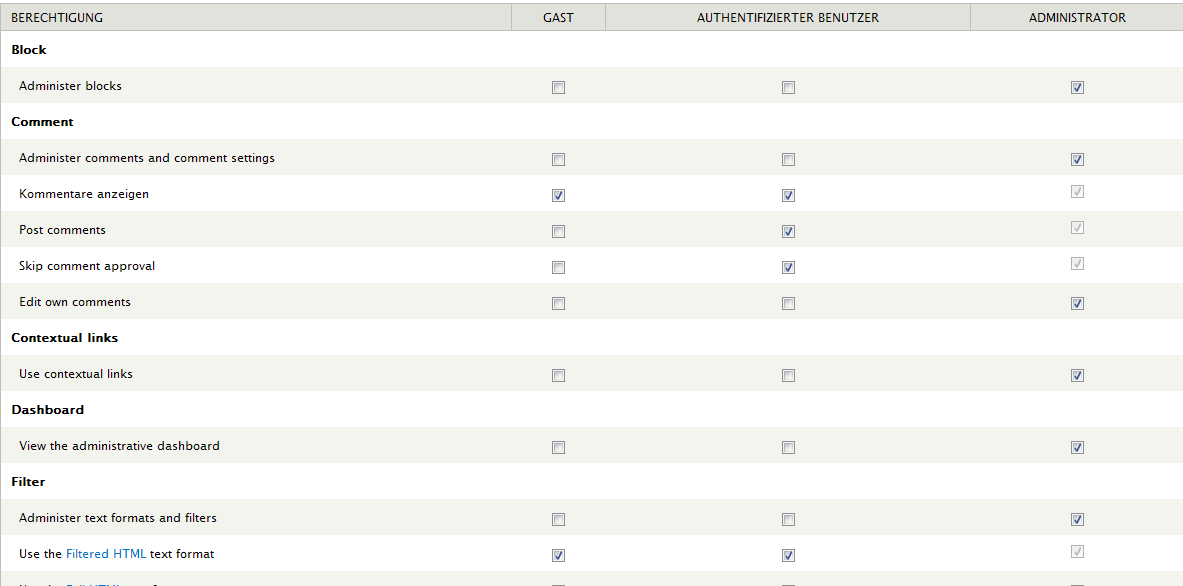
\includegraphics[width=\textwidth]{img/drupal_rollensystem.png}
\caption{Ausschnitt aus rechtebasiertem Rollensystem von Drupal}
\label{fig:drupal_rollen}
\end{figure}
\begin{figure}[ht]
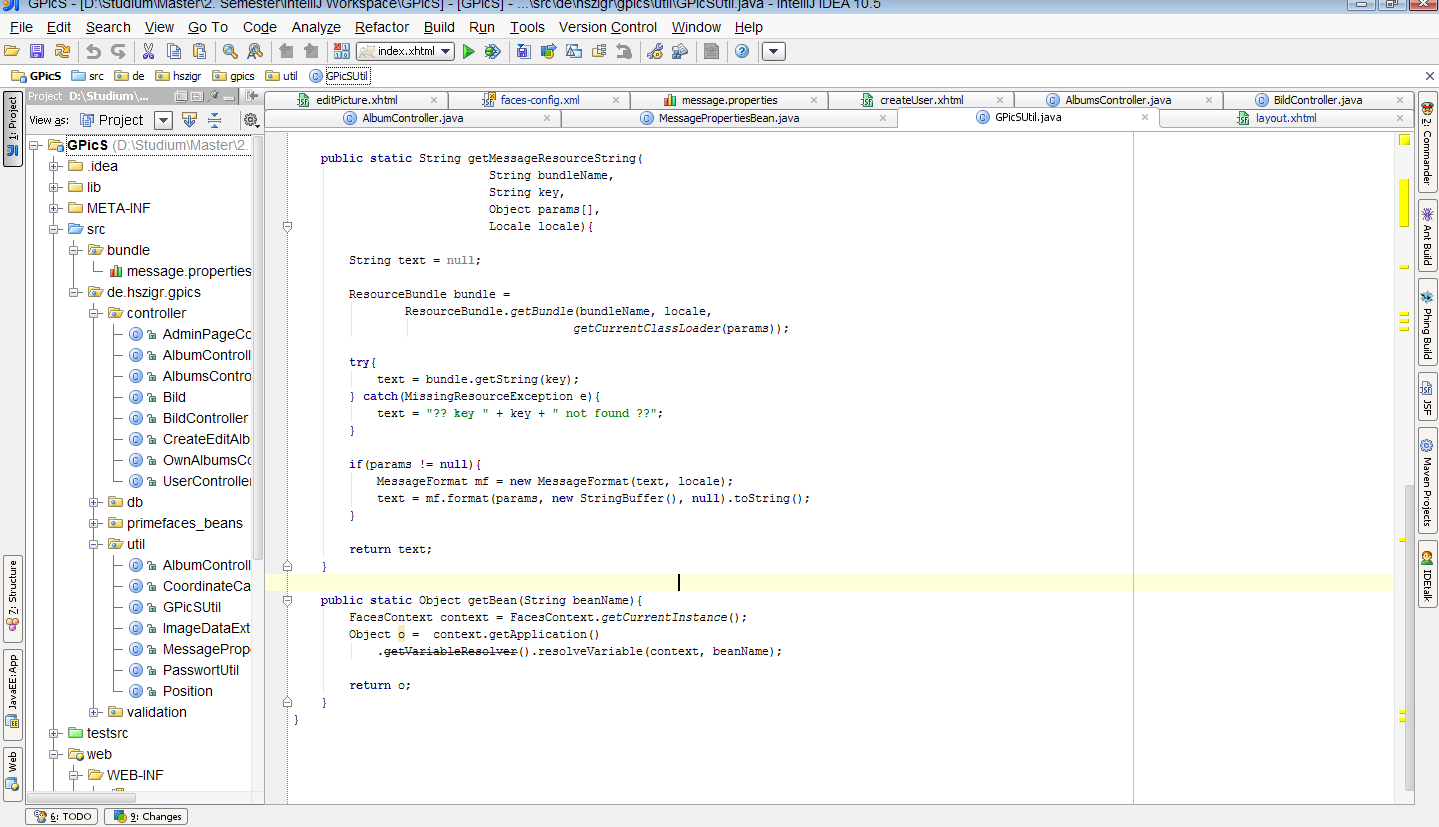
\includegraphics[width=\textwidth]{img/intellij_toolmenu.png}
\caption{Menues rund um den Quellcode}
\label{fig:intellij_menu}
\end{figure}
	\newpage
	\input{Eidesstattliche-Erkl�rung}
\end{document}